%%%%%%%%%%%%%%%%%%%%%%%%%%%%%%%%%%%%%%%%%%%%%%%%%%%%%%%%%%%%%%%%%%%%%%%%%%
%
% StEvent - User Guide and Reference Manual -- LaTeX Source
%
% $Id: StEvent.tex,v 2.6 1999/11/22 20:58:43 ullrich Exp $
%
% Author: Thomas Ullrich, Nov 1999
%
%%%%%%%%%%%%%%%%%%%%%%%%%%%%%%%%%%%%%%%%%%%%%%%%%%%%%%%%%%%%%%%%%%%%%%%%%%
%
% Notes to the authors:
%
% - A template for a class reference is at the end of this file.
% - Wrap all names functions with \name{}
% - All code, examples, prototypes in \verb+ ... +\\
%   or /begin{verbatim} ... \end{verbatim}
% - Use \StEvent if you refer to the package itself (not the class)
%
% This file is best edit with xemacs and the 'Function' package loaded.
%
%%%%%%%%%%%%%%%%%%%%%%%%%%%%%%%%%%%%%%%%%%%%%%%%%%%%%%%%%%%%%%%%%%%%%%%%%%
%
% $Log
% Revision 2.33  2000/05/22 22:04:07  ullrich
% Removed StRichPixelCollection ref section and added description
% of new RICH methods to class StEvent.
%
% Revision 2.45  2000/08/23 03:14:07  ullrich
% Improved (corrected) explanation of return value
% of chi2 methods of StVertex and StTrackFitTraits.
%
% Revision 2.44  2000/08/17 00:36:31  ullrich
% Added description of StTptTrack.
%
% Revision 2.43  2000/08/17 01:18:02  ullrich
% Fixed wrong description of StZtbTriggerDetector::adc().
%
% Revision 2.42  2000/07/13 12:47:07  ullrich
% Added ZDC info provided by Clemens
%
% Revision 2.41  2000/06/29 18:00:37  ullrich
% Better description of StCtbTriggerDetector.
%
% Revision 2.40  2000/06/22 18:18:33  ullrich
% Fixed problem with page numbering. Increased textheight.
%
% Revision 2.39  2000/06/21 22:55:42  ullrich
% Added StEventInfo to ref section. Updated StEvent.
%
% Revision 2.38  2000/06/07 09:44:20  ullrich
% Modified StHit ref section.
%
% Revision 2.37  2000/06/01 21:36:17  ullrich
% Added new method flag() to StHit description.
%
% Revision 2.36  2000/06/01 16:46:23  ullrich
% Mods (add text) in StTrack and StTrackDetectorInfo.
%
% Revision 2.35  2000/05/31 14:26:26  lasiuk
% Add RICH classes and descriptions
%
% Revision 2.32  2000/05/17 17:20:01  ullrich
% Updates and improved description of StTrackTopologyMap.
% Revision 2.31  2000/05/16 13:22:39  ullrich
% More details on the second chi2 value in StTrackFitTraits.
%
% Revision 2.30  2000/05/09 11:09:30  ullrich
% Updated section on StMwcTriggerDetector and StCtbTriggerDetector.
%
% Revision 2.29  2000/04/26 21:01:44  ullrich
% Removed text for obsolete StBrowsableEvent.
%
% Revision 2.28  2000/04/20 13:31:25  ullrich
% Added description of changes to StTrackDetectorInfo.
%
% Revision 2.27  2000/04/10 19:59:34  genevb
% StRoot/StEvent/doc/tex/
%
% Revision 2.26  2000/03/30 16:55:38  ullrich
% Modified reference section for StTrack::key().
%
% Revision 2.25  2000/03/29 16:55:48  ullrich
% Added reference section and emprt user guide page for StL3Trigger.
%
% Revision 2.24  2000/03/23 18:30:50  ullrich
% Added new EMC classes to reference section.
%
% Revision 2.23  2000/03/08 14:27:45  ullrich
% Added description of new method of StVertex.
%
% Revision 2.22  2000/03/02 12:40:40  ullrich
% Added description of modified StTpcDedxPidAlgorithm
%
% Revision 2.21  2000/02/28 19:37:26  ullrich
% Added the hypperref package to add bookmarks and hyperlinks
% tp pdf documents.
%
% Revision 2.20  2000/02/24 13:25:12  ullrich
% Added RICH and EMC to the reference section. Created
% (empty) section for EMC and RICH in User Guide.
% Revision 2.19  2000/02/17 18:16:18  ullrich
% Add documentation of new SVT hit storage layout.
%
% Revision 2.18  2000/02/11 16:23:45  ullrich
% Add info on order in which primary vertices are stored
% and added description of StPrimaryVertex::flag().
%
% Revision 2.17  2000/01/31 13:40:40  ullrich
% Added Helens description of iflag (see StTrack::flag()).
%
% Revision 2.16  2000/01/27 18:38:30  ullrich
% Fixed typo in units for curvature.
%
% Revision 2.15  2000/01/12 10:45:31  ullrich
% Fixed error (underscore in text).
%
% Revision 2.14  2000/01/11 16:31:56  ullrich
% Regular update.
%
%%%%%%%%%%%%%%%%%%%%%%%%%%%%%%%%%%%%%%%%%%%%%%%%%%%%%%%%%%%%%%%%%%%%%%%%%%
\documentclass[twoside]{article}

\parindent 0pt
\parskip 6pt
\advance\textheight by 80pt%
\advance\textwidth by 80pt%
\advance\evensidemargin by -80pt%

\usepackage{graphicx}
\usepackage{psboxit}
\usepackage{amsmath}
\usepackage{amssymb}
\usepackage{amsfonts}
\usepackage{fancyhdr}
\usepackage{times}
\usepackage{verbatim}
\usepackage{makeidx}
\usepackage[dvips=true,hyperindex=true,colorlinks=true,linkcolor=blue,bookmarks=true]{hyperref}

\PScommands      % init boxit
\makeindex

%%%%%%%%%%%%%%%%%%%%%%%%%%%%%%%%%%%%%%%%%%%%%%%%%%%%%%%%%%%%%%%%%%%%
%
% Define header and footer style
  {\LARGE $ $Revision: 2.6 $ $}  \\[5mm] % replaced by cvs with current revision
  {\LARGE $ $Date: 1999/11/22 20:58:43 $ $}  % replaced by cvs with current revision
\pagestyle{fancyplain}
\rhead[\fancyplain{}{\bfseries\leftmark}]
      {\fancyplain{}{\bfseries\rightmark}}
\lhead[\fancyplain{}{\bfseries\rightmark}]
      {\fancyplain{}{\bfseries\leftmark}}
\rfoot[{}]{\fancyplain{}{\bfseries\thepage}}
\lfoot[\fancyplain{}{\bfseries\thepage}]{}
\cfoot{}

%%%%%%%%%%%%%%%%%%%%%%%%%%%%%%%%%%%%%%%%%%%%%%%%%%%%%%%%%%%%%%%%%%%%
%
% Typographic Conventions
%
%%%%%%%%%%%%%%%%%%%%%%%%%%%%%%%%%%%%%%%%%%%%%%%%%%%%%%%%%%%%%%%%%%%%
\newcommand{\name}[1]{\textsl{#1}}%  class-, function-, package names
\newcommand{\StEvent}{\textsf{StEvent}}

%%%%%%%%%%%%%%%%%%%%%%%%%%%%%%%%%%%%%%%%%%%%%%%%%%%%%%%%%%%%%%%%%%%%
%
% Define multiline labels for class reference
%
%%%%%%%%%%%%%%%%%%%%%%%%%%%%%%%%%%%%%%%%%%%%%%%%%%%%%%%%%%%%%%%%%%%%
\newcommand{\entrylabel}[1]{\mbox{\textbf{{#1}}}\hfil}%
  {\LARGE $ $Revision: 2.6 $ $}  \\[5mm] % replaced by cvs with current revision
  {\LARGE $ $Date: 1999/11/22 20:58:43 $ $}  % replaced by cvs with current revision
    {\renewcommand{\makelabel}{\entrylabel}%
     \setlength{\labelwidth}{90pt}%
     \setlength{\leftmargin}{\labelwidth}
     \advance\leftmargin by \labelsep%
      }%
    }%
  {\end{list}}
  {\LARGE $ $Revision: 2.6 $ $}  \\[5mm] % replaced by cvs with current revision
  {\LARGE $ $Date: 1999/11/22 20:58:43 $ $}  % replaced by cvs with current revision
\index{header files}
\index{StEventTypes.h file}
    {\parbox[t]{\labelwidth}{\hspace{0pt}\textbf{{#1}}}}}}
\newenvironment{Entry}%
{\renewcommand{\entrylabel}{\Entrylabel}\begin{entry}}%
where-ever possible forward declarations were used.  This is
especially true for the StEvent class itself and it is therefore
\emph{not} sufficient to include \texttt{StEvent.h} only.  Many more
header files would have to be included. This is very good for the
developers since turnaround times are minimized but obviously bad for
the users for it would be very cumbersome to each time figure out
which header files one might need and which not. Therefore are
\emph{all} header files needed to use every little bit of \StEvent\ 
put together in one single file: \texttt{StEventTypes.h}.  The
disadvantage of this approach is that every time one \StEvent\ class
changes you have to recompile all your code, even if the changed class
is not used. This, however, should not happen too often and it by far
more convenient to deal with on header file only.
  {\Large\bf STAR Offline Library Long Writeup}
To summarize: All you need when using StEvent is to include
  \mbox{\includegraphics[width=\textwidth]{StEventTitle.eps}}
  \hfill\mbox{}\\[3cm]
  {\LARGE User Guide and Reference Manual \\[5mm] for Version 2}\\[2cm]
  {\LARGE $ $Revision: 2.6 $ $}  \\[5mm] % replaced by cvs with current revision
\index{enumerations}
\index{constants}
\index{StDetectorId.h file}
\index{StVertexId.h file}
\index{StEnumerations.h file}

\StEvent\ uses a lot of enumeration for all types of purposes. This
is much more type-safe then using simple integer numbers and makes the
code much more readable. All enumerations used in \StEvent\ are defined
in \texttt{StEnumerations.h}. 
For users convenience also the ``standard'' header files
\texttt{StDetectorId.h}, \texttt{StVertexId.h} and \texttt{StTrackMethod.h}
are included therein.
%    Table of content
%
%%%%%%%%%%%%%%%%%%%%%%%%%%%%%%%%%%%%%%%%%%%%%%%%%%%%%%%%%%%%%%%%%%%%
\tableofcontents
\cleardoublepage

To remind you of the names and save you the time to look them up
every time they are all listed below:
%    Introduction
%
%%%%%%%%%%%%%%%%%%%%%%%%%%%%%%%%%%%%%%%%%%%%%%%%%%%%%%%%%%%%%%%%%%%%


\StEvent\ version 2. Like the new version of \StEvent\ this
with revision number 1.xx. All code and documentation for the new

In this document more emphasis is put on the User Guide while the
Reference Manual part is kept shorter in terms of description of
usage.  As \StEvent\ changes this document will change accordingly and
you should always check that the revision number of the document
matches the one in the repository.

Version 2 of \StEvent\ contains significant changes as compared to the
previous versions. Part of the changes were made to cope with the
modification of the DST format in Fall of 1999, others were made to
overcome shortcomings in the previous implementation. This version is
\pagenumbering{arabic}
also more flexible in terms of extendibility to allow future track and
vertex models to be incorporated easily.  The current implementation
is also meant to be used further upstream of the analysis, i.e. in the
reconstruction phase.  As a consequence the model itself became
slightly more complex in terms of navigation and structuring.

In order to explain the model in practical terms many diagrams and
plots were included in this document. Some of them show class diagrams
using the Unified Modelling Language UML. A brief introduction to UML
is given in Appendix~\ref{sec:introUML}.\index{UML}
\begin{figure}[hb]
    \begin{center}
        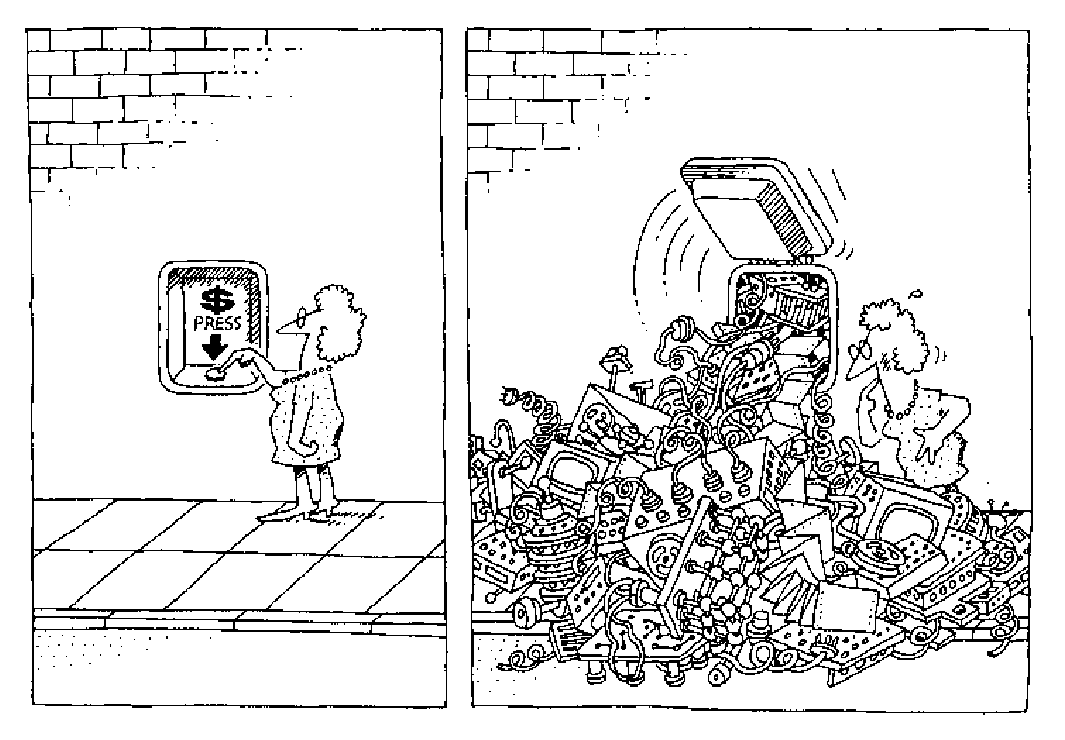
\includegraphics[width=0.9\textwidth]{cartoon1.eps}
            engineer the illusion of simplicity.}
    \end{center}
\end{figure}

\clearpage

enum StDedxMethod           {kUndefinedMethodId,       
                             kTruncatedMeanId,         
                             kEnsembleTruncatedMeanId, 
                             kLikelihoodFitId,         
                             kWeightedTruncatedMeanId, 
\clearpage
enum StTrackFindingMethod   {kUndefinedFinderId,         
                             kSvtGrouperId,
                             kSvtStkId,
                             kTpcStandardId,
                             kSvtTpcSvmId,
                             kSvtTpcEstId};                          
enum StTrackQualityScheme   {kUndefinedQualityId,        
                             kGrouperPassId,
                             kStkPassId,
                             kSvmPassId,
                             kEstPassId};                                                      
enum StTrackFittingMethod   {kUndefinedFitterId,         
\label{sec:Basics}

\subsection{Header Files}
\label{sec:HeaderFiles}
\index{header files} \index{StEventTypes.h file}
\emph{all} header files which are needed to use every little bit of
\StEvent\ contained in one single header file named
\texttt{StEventTypes.h}.  The disadvantage of this approach is that
are used as an argument types. The strong C++ type
checking rules ensures the proper use of the enumeration
constants already during compilation.

Another important set of constants should be mentioned here as well, namely
the physical constants as defined in \texttt{PhysicalConstants.h}.
There are too many to be listed here but you should make yourself familiar
with what is available. You will find it in the \name{StarClassLibrary}
(see Sec.~\ref{sec:furtherDoc}). \index{StarClassLibrary}
In order to define the units of the various physical constants another set
of constants defined in \texttt{SystemOfUnits.h} is used (also from 
\name{StarClassLibrary}). The latter is described in section \ref{sec:units}.
\StEvent\ uses a lot of enumerations for all types of purposes. This
is much more type-safe then using simple integer numbers and makes the
code more readable. All enumerations used in \StEvent\ are defined in
\texttt{StEnumerations.h}.  For users convenience some non-\StEvent\
header files as \texttt{StDetectorId.h}, \texttt{StVertexId.h} and
\subsubsection{Numbering Scheme}
enum StTrackType            {global, primary, secondary};
All numbering follows \emph{strictly} the C/C++ convention. This
includes not only indices as usual but also for example sector
numbers, row numbers and wafer numbers. If you follow this rule things
become less confusing for there is only one way of counting. This
allows to follow the usual C/C++ syntax in all forms:
\begin{verbatim}
const int nSectors = 24;
for (int i=0; i<nSectors; i++)
    // ...
\end{verbatim}
If you find a deviation from this rule it is a bug.
                             kEndcapEmcPreShowerId,
                             kEndcapSmdEtaStripId,
\index{references}
\index{pointers}
                             kZdcWestId,
Many methods (or member functions) or \StEvent\ classes return
objects by \emph{reference} or by \emph{pointer}. This is sometimes confusing
but there is a idea behind this. Whenever an object is returned
by reference it is guaranteed to exist. No questions asked. If the
object is a container it might be empty, i.e. it has zero size,
but you ask for it you get it. Objects returned by pointer, however,
are \emph{not} guaranteed to exist. You might get a NULL pointer back.
It is always a good idea to check if you really get what you asked
for. Dereferencing a NULL pointer can be painful.

As you will see in the reference sections many methods are provided
in two versions: a constant and a non-constant version. Don't worry
about the differences. The compiler will always choose the proper
version.
                             kOtherVtxId};

enum StDedxMethod           {kUndefinedMethodId,
\index{units}
\index{system of units}
All physics quantities in \StEvent\ are stored using the official STAR
units: cm, GeV and Tesla.  Angles are given in radians\footnote{Note,
    that here \StEvent\ deviates from STAR guidelines where degrees
    are declared the official units.}  In order to maintain a coherent
system of units it is recommended to use the definitions in
\texttt{SystemOfUnits.h} from the StarClassLibrary. They allow to
'assign' a unit to a given variable by multiplying it with a constant
named accordingly (centimeter, millimeter, kilometer, tesla, MeV,
...).  The value of the constants is thus that the result after the
multiplication follows always the STAR system of units.

                             tpcOther,
                             ftpcConformal,
                             svtTpcSvm,
                             svtTpcEst,
                             svtTpcPattern};

enum StRichPidFlag          {eNoMip,
                             eFastEnough,
                             eLightOnPadPlane};
\end{verbatim}

Note that often the enumeration type names (e.g. \texttt{StTrackType})
are used as argument types. The strong C++ type checking rules ensures
the proper use of the enumeration constants already during
compilation.

Another important set of constants should be mentioned here as well,
namely the physical constants defined in \texttt{PhysicalConstants.h}.
There are too many to be listed here but you should make yourself
familiar with what constants are available. You will find the header
file in the \name{StarClassLibrary} (see Sec.~\ref{sec:furtherDoc}).
\index{StarClassLibrary} In order to define the units of the various
physical constants another set of constants defined in
\texttt{SystemOfUnits.h} is used (also from \name{StarClassLibrary}).
The latter is described in section \ref{sec:units}.

\subsection{Conventions}
\index{conventions}
\label{sec:conventions}

\subsubsection{Numbering Scheme}
\label{sec:conventionsNumbering}

All numbering follows \emph{strictly} the C/C++ convention, i.e. the
first element in an array has the index 0. This is valid for all
container, collections and lists. Here it is important to remember
that many (but not all) official STAR numbering schemes start counting
at 1.  Examples are TPC sectors and padrows, SVT barrels, layers, ladders and
wafers. Do not forget to subtract 1 when using this scheme for
addressing elements in a container.

TPC, SVT and FTPC hits return their hardware address in STAR units.
In order to select the hit container in which a hit \texttt{h} is
stored you must write:
Further documentation can be found in the StarClassLibrary manual
(see Sec.~\ref{sec:furtherDoc}).\vfill
\end{verbatim}

programming language and C/C++ played only a minor role. Again, the only
\index{ROOT}
\index{persistence}
All \StEvent\ classes inherit from \texttt{StObject} which itself inherits
from \texttt{TObject}. During the build of \StEvent\ all classes run through
\texttt{rootcint}. This adds the following features:
\item \texttt{StTpcHit::padrow()}
\item All \StEvent\ classes can be used on the \texttt{root4star} command line.
\item Almost all \StEvent\ classes are persistent capable, i.e. they can be stored
    in ROOT files.
\item \textrm{StSvtHit::wafer(})
As usual each coin has two sides. The disadvantage of this is that we cannot use
some features of the ANSI/ISO C++ and from the Strandard C++ Library as:
\end{itemize}
See the corresponding reference sections for more.
\item templates 
\item STL containers and algorithms    
\item namespaces    

This however applies for the header files only. Source files are not processed
via \texttt{rootcint} and therefore all the stuff mentioned above can be used.
And indeed in the implementation of various \StEvent\ classes we make heavily
use of STL features.
is a container it might be empty, i.e. it has zero size, but you ask
for it you get it. Objects returned by pointer, however, are
\emph{not} guaranteed to exist. You might get a \texttt{NULL} pointer
back.  It is always a good idea to check if you really get what you
asked for.  Dereferencing a \texttt{NULL} pointer can be painful.

As you will see in the reference section many methods are provided in
two versions: a constant and a non-constant version. Don't worry about
ROOT uses typedefs for the builtin standard C++ types. This is pretty confusing
but has a good reason when it comes to persistence. This way one can guarantee the
same size (number of bytes) for the types independent of the platform. 
The ANSI/ISO standard only requires that:
\texttt{char} $\le$ \texttt{short} $\le$ \texttt{int} $\le$ \texttt{long} $\le$ \texttt{long long}
and 
\texttt{float} $\le$ \texttt{double} $\le$ \texttt{long double}.
units: cm, GeV and Tesla.  Angles are given in radians\footnote{Note,
    that here \StEvent\ deviates from STAR guidelines where degrees
    are declared the official units.}  In order to maintain a coherent
system of units it is recommended to use the definitions in
\texttt{SystemOfUnits.h} from the \name{StarClassLibrary}. They allow
to 'assign' a unit to a given variable by multiplying it with a
constant named accordingly (centimeter, millimeter, kilometer, Tesla,
MeV, ...).  The constants ensure that the result after the
multiplication follows always the STAR system of units.

The following example illustrates their use:
\begin{verbatim}
double a = 10*centimeter;
typedef unsigned char  Bool_t;      //Boolean 
double c = 1*inch;
double E1 = 130*MeV;
double E2 = .1234*GeV;

//
and speed. It also makes code less portable and readable.
Don't use them only because you see them used in \StEvent.
cout << "STAR units:" << endl;
cout << "a = " << a << " cm" << endl;
cout << "b = " << b << " cm" << endl;
\index{container}
\index{iterators}
Version 2 of \StEvent\ comes with a new naming scheme for containers.
All containers used in \StEvent\ store objects by pointer. Technically
they are all vectors and therefore allow random-access as in
//
//   Print in personal units
//
that is they are ordered collections. There are two different types
of containers, so called structural and non-structural containers.
What that means is rather simple. Structural containers \emph{own}
the objects they contain the others not. If you delete a structural
cout << "E1 = " << E1/TeV << " TeV" << endl;
cout << "E2 = " << E2/keV << " keV" << endl;
\end{verbatim}
The resulting printout is:
\begin{verbatim}
STAR units:
a = 10 cm
b = 0.4 cm
c = 2.54 cm
E1 = 0.13 GeV
E2 = 0.1234 GeV

My units:
a = 100 mm
and non-structural collection. Their interface is the same and they
act they same. The secret lies in their implementation. If you create
a container by your own you should always use the non-structural
containers. Those you van create and delete without doing \StEvent\ 
\end{verbatim}
your back to wall with a sharp knife on your throat.
manual (see Sec.~\ref{sec:furtherDoc}).\vfill
All containers used in \StEvent\ are defined in the \texttt{StContainers.h} header
file and are based on StArray which was written by Victor Perevoztchikov.
\index{StContainers.h}
\label{sec:Persistence}
\index{ROOT} \index{persistence} All \StEvent\ classes inherit from
\texttt{StObject} which itself inherits from \texttt{TObject}. During
the build of \StEvent\ all classes run through \texttt{rootcint}. This
adds the following features:
\begin{enumerate}
\item All \StEvent\ classes can be used on the \texttt{root4star}
    command line.
\item Almost all \StEvent\ classes are persistent capable, i.e. they
    can be stored in ROOT files.
\end{enumerate}
As usual each coin has two sides. The disadvantage of this is that we
cannot use some features of the ANSI/ISO C++ and from the Standard C++
Library as:
\begin{itemize}
\item type bool
\item templates
\item STL containers and algorithms
\item namespaces
All containers are based on modified ROOT \index{ROOT} collections. They
allow to make \StEvent\ persistent. They good thing with \texttt{StArray}
is that all those containers offer an almost ANSI/ISO compatible interface.
This means that \emph{both} containers classes provide the essential methods
listed below. Replace \texttt{ClassName} with whatever \StEvent\ class.
    \begin{center}
        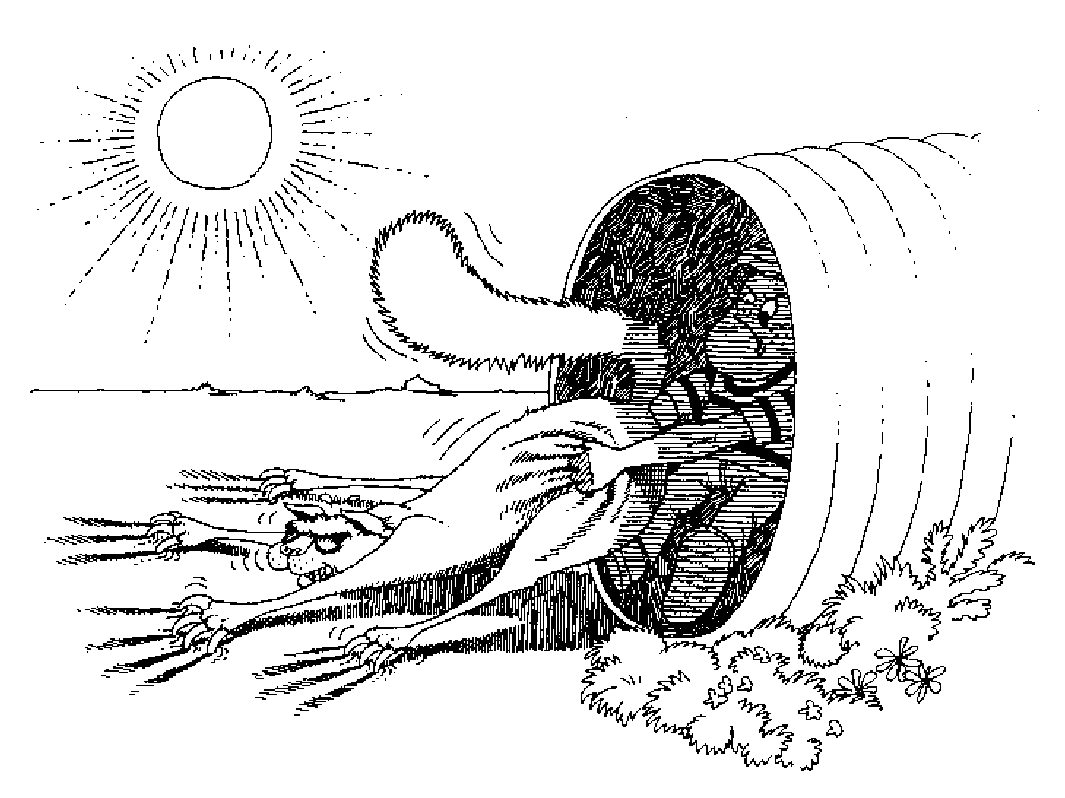
\includegraphics[width=0.5\textheight]{cartoon4.eps}
        \caption{Persistence saves the state and class of an object
            across time or space.}
    \end{center}
\end{figure}

ROOT uses typedefs for the built-in standard C++ types. This is pretty
confusing but has a good reason when it comes to persistence. This way

independent of the platform.  The ANSI/ISO standard only requires
that: \texttt{char} $\le$ \texttt{short} $\le$ \texttt{int} $\le$
    Copy constructor. Structural containers copies also the
    objects it contains.

The types used in \StEvent\ are defined as follows:
\begin{verbatim}
    Adds object pointed to by \texttt{pobj}. If the container is not large
    enough it will automatically resize.
typedef short          Short_t;     //Signed Short integer 2 bytes
typedef unsigned short UShort_t;    //Unsigned Short integer 2 bytes
    Returns the current size of the container, i.e. the number
    of stored elements.

typedef unsigned long  ULong_t;     //Unsigned long integer 4 bytes
typedef float          Float_t;     //Float 4 bytes
typedef double         Double_t;    //Float 8 bytes
typedef unsigned char  Bool_t;      //Boolean
    Deletes all elements.

code other than in the definition of class data member. Even worse
this can have disadvantages when it comes to calls to system functions
and speed. It also makes code less portable and readable.  Don't use
them only because you see them used in \StEvent.

\subsection{Container and Iterators}
\label{sec:Container}
\index{container} \index{iterators} Version 2 of \StEvent\ comes with
a new naming scheme for containers.  All containers used in \StEvent\
store objects by pointer. Technically they are all vectors and
therefore allow random-access as in
\begin{verbatim}
    pointer_to_object = container[i];
    Deletes element referred to by iterator \texttt{iter}.
    If applied to structural containers the objects gets deleted.
containers, so called structural and non-structural containers.  What
that means is rather simple. Structural containers \emph{own} the
objects they contain the others not. If you delete a structural
container all objects stored in it get deleted as well.
\begin{itemize}
\item All \textbf{s}tructural \textbf{vec}tors which store
There are many more than one can describe here.
If you want to learn more you better have a look at the
\texttt{StArray.h} source code directly.
    \textbf{p}oin\textbf{t}e\textbf{r}s carry the prefix
Needless to say that every container comes with two iterators a
constant and a non-constant version.  The name of each iterators is
composed of the name of container and the
contain and we are done. Hence a structural container which holds
objects (or better pointer to objects) of type \texttt{StTrackNode} is
iterators StSPtrVecTrackNodeIterator and
StSPtrVecTrackNodeConstIterator are defined.  Iterators care if the
iterate over about structural or non-structural containers so there
are two sets of iterators for \texttt{StSPtrVecTrackNode} and
they same. The secret lies in their implementation. If you create a
container by your own you should always use the non-structural
containers. Those you can create and delete without doing \StEvent\
any harm. Never delete a structural container unless you stand with
your back to a wall and a sharp knife on your throat.
version has some advantages and is safer.
All containers used in \StEvent\ are defined in the
\texttt{StContainers.h} header file and are based on \texttt{StArray}
which was written by Victor Perevoztchikov.  \index{StContainers.h}
Currently the following containers are in use:
\begin{verbatim}
StPtrVecHit
StPtrVecTrack
StPtrVecTrackPidTraits
StSPtrVecFtpcHit
StSPtrVecKinkVertex
StSPtrVecPrimaryTrack
StSPtrVecPrimaryVertex
StSPtrVecSvtHit
StSPtrVecTpcHit
A warning at the end. Although StArray provides a interface compatible
with the Standard C++ Library (former STL) it is not guaranteed that
the standard algorithms will work (\texttt{sort}, \texttt{accumulate},
\texttt{copy}, \texttt{find}, ...). You better check this from case to
case. Don't say you haven't been warned.

For your own analysis (or reconstruction) code you might use the standard
STL containers together with StEvent freely provided that you classes are not
processed via \texttt{rootcint}. Since STL containers are transient they
are more efficient if speed and use less memory if this is your concern.
compatible interface.  This means that \emph{both} container classes
provide the essential methods listed below. Replace \texttt{ClassName}
with any \StEvent\ class one might find in a container.
\begin{Entry}
\item[Public\\ Constructors]
    \verb+StPtrVecClassName();+\\
    \verb+StSPtrVecClassName();+\\
    Constructs an instance with zero length.

    \verb+StPtrVecClassName(UInt_t nelem);+\\
    \verb+StSPtrVecClassName(UInt_t nelem);+\\
    Constructs an instance with length \texttt{nelem}.
    
    \verb+StPtrVecClassName(const StPtrVecClassName& vec);+\\

    Copy constructor. Structural containers copy also the objects they
    contain.
    
\item[Public Member\\ Functions]
    \verb+Bool_t  doLoadFtpcHits;+\\   
    Adds object pointed to by \texttt{pobj}. If the container is not

    \verb+Bool_t  doLoadSvtHits; +\\   
    \verb+UInt_t size() const;+\\
    Returns the current size of the container, i.e. the number of
    \verb+Bool_t  doPrintRunInfo;+\\   
    Print or do not print dump of current instances of StRun and
    StRunSummary (default=kFALSE).    


    Print or do not print info on the current StEvent
    Deletes all elements. If the container is a structural container
    all objects it holds get deleted.
    element in every container (default=kFALSE). Don't use it for
    production. 

    Checks for zero size.
    Switch on/off checks on memory usage of StEvent (default=kFALSE).
    In order to get a memory snapshot we uses \texttt{StMemoryInfo}
    from the \name{StarClassLibrary}.  A snapshot is taken before and
    after the setup of StEvent and StRun.  The numbers in brackets
    refer to the difference. Not available on SUN Solaris.
    \verb+const StSPtrVecClassNameIterator end() const;+\\
    Returns iterator to the the last+1 element in the collection.
    
    took to setup StEvent. Timing is performed using \texttt{StTimer}
    \verb+void erase(StSPtrVecClassNameIterator iter) const;+\\
    Deletes element referred to by iterator \texttt{iter}.  If applied
    to structural containers the object gets also deleted.
    
    Returns a pointer to the current StEvent object. The object
    returned is actually of type \texttt{StBrowsableEvent}.
    Returns the pointer to the \texttt{i}'th element where \texttt{i}
    runs from 0 to \texttt{size()-1}.
    Returns a pointer to the current StRun object.
    This object is only updates for a new run, else you will
    get always the same instance.

Needless to say that every container comes with two iterators, a
constant and a non-constant version.  The name of each iterator is
composed of the name of the container and the
suffix \texttt{Iterator} or \texttt{ConstIterator}.\\
Example: For the structural container \texttt{StSPtrVecTrackNode} the
iterators \texttt{StSPtrVecTrackNodeIterator} and
\texttt{StSPtrVecTrackNodeConstIterator} are defined. Iterators care
if they iterate over structural or non-structural containers so there
are different iterators for \texttt{StSPtrVecTrackNode} and
\texttt{StPtrVecTrackNode} containers.
\index{doEvents.C}
\index{StEventMaker}
\index{StAnalysisMaker}
\index{root4star}
\index{ROOT files}
\index{XDF files}
In order to get started it is always a good idea to study a
simple example which shows the essential steps on how to
analyse data using \StEvent.
The procedure starting from scratch to run the provided StEvent usage
example is
StPtrVecTrack container;
float x;

\\ method 1
for (unsigned int i=0; i<container.size(); i++)
      x = container[i]->length();

\\ method 2
for (StPtrVecTrackIterator i = container.begin(); i != container.end(); i++)
      x = (*i)->length();
\end{verbatim}

A warning at the end. Although \texttt{StArray} provides a interface
compatible with the Standard C++ Library (former STL) it is not
guaranteed that the standard algorithms will work (\texttt{sort},
\texttt{accumulate}, \texttt{copy}, \texttt{find}, ...). You better
check this from case to case. Don't say you haven't been warned.

For your own analysis (or reconstruction) code you might use the
standard STL containers together with \StEvent\ provided that you
\item[\texttt{StAnalysisMaker}:] Pick up the \texttt{StEvent} event and analyze it
    (incorporates a few simple examples).
are transient they are more efficient if speed and use less memory if
this is your concern.
specified root directory (see doEvents.C for details), eg. example
\subsection{Getting StEvent: The StEventMaker}
\label{sec:StEventMaker}
\index{StEventMaker}

\StEvent\ is set up and filled in a ``maker'' with the name
\texttt{StEventMaker}.  This maker reads DST tables stored in memory
and does all the things to make \StEvent\ nice and useful. How the DST
gets into memory is another story and is explained in the next section
    \verb+Bool_t  doPrintRunInfo;+\\
\begin{Entry}
    
\item[Public Data\\ Member]
    \verb+Bool_t  doLoadTpcHits;+\\
it yourself you can pick up StAnalysisMaker and modify it piece by
piece or use it as a template for a Maker of your own that works with
StEvent:
    Controls if FTPC hits should be loaded (default=kTRUE).
    
    \verb+Bool_t  doLoadSvtHits; +\\
    Controls if SVT hits should be loaded (default=kTRUE).
    [and edit and modify]
    \verb+Bool_t  doLoadTptTracks;+\\
    Controls if TPT tracks should be loaded (default=kFALSE).
    [and edit to use your maker]
    root4star doEvents.C
    Print or do not print info on the current \StEvent\ event.
By the time you gain more experience your ``maker'' will become more and
more sophisticated but the basic idea shown in the example stays the same.
    
    \verb+Bool_t  doPrintMemoryInfo;+\\
    Switch on/off checks on memory usage of \StEvent\
\index{documentation}
All documentation specific to the various packages is under cvs
control and stored in the same repository as the source code of the
package. You will find it usually in a directory called \texttt{doc}.
In addition to that every package should contain a \texttt{README} and
a \texttt{index.html} file with further information. (Note the
``should''.) 

\StEvent\ makes use of various classes from the StarClassLibrary
(SCL).  Examples are \texttt{StThreeVector}, \texttt{StHelix} and
\texttt{StParticleDefinition}. You should have a version of the
corresponding LaTeX manual at hand.\index{SCL} \index{StarClassLibrary}
    \verb+StRun*    run();+\\
    Returns a pointer to the current \texttt{StRun} object.  This
    object gets only updated for a new run, else you will get always
    the same instance.
reflects this content (although in a different way and approach) this is
the place to check if you don't understand the meaning of certain
variables or methods.  In this manual we cannot go too much into every
detail.
mentioned here: Do \emph{not} delete the \texttt{StEvent} or
And finally you really should have the C++ bible from B.~Stroustrup
within 100 feet distance from your desk. The more you get into C++ and OO
the more you will appreciate this book. We already mentioned that

the internal structure you will find things like virtual constructors,
overloaded new/delete operators and much more.
Then it is nice to have Bjarnes book around to look things up.
\index{Stroustrup, Bjarne}
\clearpage

In order to get started it is always a good idea to study a simple
In the following we describe the basic concepts of \StEvent.
This is not to describe every class and every method but to explain
the idea behind it and illustrate a few things in examples.
If you need more details have a look at the reference section and if
you want to know \emph{everything} about \StEvent\ you have to visit
the source code directly.
    root4star
\end{verbatim}
\index{StRun}
\index{StRunSummary}
\index{run header}
\index{run summary}
The class \texttt{StRun} contains all information you would expect
from a run header: run number, trigger settings, beam setup, and
much more. Every living \texttt{StRun} object also contains a pointer to an
instance of \texttt{StRunSummary} which contains - you guessed it - the run summary.
The fact that the summary is contained by pointer already tells
you that the pointer might be \texttt{NULL} if something went wrong.
So better make sure it is non-zero before you de-reference it.\\
The run summary contains information gathered during the DST reconstruction like
average pt, average pseudo-rapitity, CPU time, and similar stuff.
It does \emph{not} contain all data on the experimental run but only on the events
of the run which were handled in a single batch job. This are usually around 50 events,an experimental run can contain thousands of events. 
It runs the chain on either a single file or all files under a
specified root directory (see doEvents.C for details). Example
invocations are:

Processes 10 events from the specified XDF file.\\
\hspace{1cm}\verb+.x doEvents.C(10,"-","/some_directory/some_dst_file.xdf");+\\

Processes 42 events from the specified ROOT file.\\
\hspace{1cm}\verb+.x doEvents.C(42,"-","/some_directory/some_dst_file.root");+\\

and \texttt{StEvent} are completely seperate entities. They don't know
specified directory.\\
i.e.~ many instances of \texttt{StEvent}.
\texttt{StEventMakerfig:umlRun} (see Sec.~\ref{sec:StEventMaker} will
give you the same one over and over again, unless there's a new run
header on the DST.

\index{example using StRun}
\index{example using StRunSummary}
Here is a small example of a function \texttt{printRunInfo} which takes
a pointer to an instance of \texttt{StRun} and prints out some stuff.
    mkdir StRoot/StMyAnalysisMaker
    cp $STAR/StRoot/StAnalysisMaker/* StRoot/StMyAnalysisMaker/
    [edit and modify]
    cons +StMyAnalysisMaker
    cp $STAR/StRoot/macros/analysis/doEvents.C ./
    [edit to use your maker]
    root4star
\end{verbatim}
At the ROOT prompt type
\begin{verbatim}
    .x doEvents.C(<your arguments>);
\end{verbatim}
By the time you gain more experience your ``maker'' will become more
and more sophisticated but the basic idea shown in the example stays
the same.

\subsection{Further Documentation}
\label{sec:furtherDoc}
\index{documentation}

In STAR all documentation specific to a packages is under cvs control
and stored in the same repository as the source code of the package.
You will find it usually in a directory called \texttt{doc}.  In
addition to that every package should contain a \texttt{README} and a
\texttt{index.html} file with further information. (Note the
properly. This code actually could have been written differently using
the \texttt{PR(x)} macro defined in \texttt{StGlobals.h} from the
StarClassLibrary.
\name{StarClassLibrary} (SCL).  Examples are \texttt{StThreeVector},
\texttt{StHelix} and \texttt{StParticleDefinition}. You should have a
one then could write\\
the helix track model used in STAR and contains many
examples.\index{SCL} \index{StarClassLibrary}

Very important is also the documentation from the
\texttt{\$STAR/pams/global/idl} area. Here you will find a detailed
description of the DST tables content.  Since StEvent pretty much
reflects this content (although in a different way and approach) this
is the place to check if you don't understand the meaning of certain
\index{event header}
\index{event summary}
\index{StEvent}
\index{StBrowsableEvent}
\index{StEventSummary}
The event header carries the same name as the whole package: \texttt{StEvent}.
Don't worry, when we talk about the package we write \StEvent, when
we talk about the class we write \texttt{StEvent}.\\
The class \texttt{StEvent} plays a special role since it is the entry point
and upper most object of the whole \StEvent\ tree. From here you can reach
every single bit and byte there is on the DST.\\
One already sees that that \texttt{StEvent} is a bit more complex than
\texttt{StRun}. However, one thing is very similar: the summary.
This is depicted in Fig.~\ref{fig:umlEvent} which shows only a very small
fraction of the class design around \texttt{StEvent}.
not to describe every class and every method in detail but to explain
the idea behind it and illustrate a few things in simple examples.  If
you need more details have a look at the reference section and if you
want to know \emph{everything} about \StEvent\ you have to visit the
source code directly.

\subsection{Run Header}
\index{StRun} \index{StRunSummary} \index{run header} \index{run
The class StEventSummary contains lots of information gathered during the
reconstruction of the event like: the number of tracks, the number of positive
or negative tracks, the number of vertices of certain types, and several
\emph{quasi}-histograms to hold for example distributions of for transverse momenta
and other essential physics quantities. The same warning as for StRun applies here.
Check the pointer to the event summary before you use it. It could be \texttt{NULL}.
went wrong. So better make sure it is non-zero before you dereference
it.\\
therefore acts the same way but it has some additional features which allow
a better integration of \StEvent\ into the ROOT framework. Since this is of no
big importance for the understanding of the data model as a whole we refer
to section \ref{sec:StEventMaker} and \ref{sec:StBrowsableEvent} for more
details.

As already mentioned StEvent opens the door to all the info there is on the DST.
In order to get there you have to navigate through the tree. Only few objects, mostly
container and collections, can be accessed directly from the StEvent objects.
Here's a list of some important objects which are directly stored in StEvent and
let you climb further down the tree:
\end{figure}
\item collection of software monitors
classes. Pretty simple.  What is not shown is the relation to the
\texttt{StEvent} class, simply because there is none.  \texttt{StRun}
and \texttt{StEvent} are completely separate entities. They don't know
\item list of all track nodes
\item list of the detector info for each track
\item primary vertices (mostly only one)
\item list of all V0 vertex candidates
\item list of all Xi vertex candidates
\item list of all kink vertex candidates
\item level-0 trigger
pointer to an instance of \texttt{StRun} as argument and prints out
And remember, an object you get \emph{by pointer} is not guaranteed to exist,
an object you get \emph{by reference} always exist.
void printRunInfo(StRun* run)
What else does \texttt{StEvent} contain? Well, all the usual stuff one would expect
to see in an event header: event identifier, time whene the event was recorded, the
trigger mask, the bunch crossing number and more. For a complete reference see
section \ref{sec:StEvent}.
    cout << "run type:              " << run->type() << endl;
    cout << "center of mass energy: " << run->centerOfMassEnergy() << endl;
    if (run->summary()) {
        cout << "# of events:            "
             << run->summary()->numberOfEvents() << endl;
        cout << "# of processed events:  "
the physics of the event but tells you a lot about how the
reconstruction programs performs. These are mostly quantities which
cannot be derived from other objects in \StEvent\ and would be lost
otherwise.  In a sense they \emph{monitor} the reconstruction details.
That's where
the name software monitor comes from.\\
\begin{figure}[htb]
allow a better integration of \StEvent\ into the ROOT framework. Since
this is of no big importance for the understanding of the data model
as a whole we refer to section \ref{sec:StEventMaker} and
\ref{sec:StBrowsableEvent} for more details.

             << run->summary()->averageLuminosity() << endl;
             << run->summary()->meanPt() << endl;
reconstruction has one. This is not really a detector but still a
large fraction of our software deals with combining all the detectors
in order to create global tracks and find the primary vertices.
This example also illustrates how useful it is to name the methods
properly. This code actually could have been written simpler using the
This is depicted in Fig.~\ref{fig:umlMonitors} where all classes and
their relations are shown.  You get the actual instance of
StSoftwareMonitor from StEvent and then you can select which
component, i.e.~which monitor object you want by invoking the proper
method. The methods are named after the component they return:
\texttt{tpc()} returns a pointer to the \texttt{StTpcSoftwareMonitor},
\texttt{svt()} to the \texttt{StSvtSoftwareMonitor} -- well, you get
the idea. As usual you should check for \texttt{NULL} pointers. If a
detector was not reconstructed in the reconstruction chain it's likely
that you will not find the corresponding monitor.

\subsection{Event Header}
They have no relation with any other class. ALl the do is to hold
data. Because of this the have no member access functions but all data
member are public. In order to make things easier for people moving
from table-based analysis to \StEvent-based analysis we kept the table
names.  With other words the software monitor classes match their
table counterparts 1:1.  The names are not always descriptive but the
author got tired of inventing new names.  You'll find more details on
what is what in the reference section of this manual.
you
can reach every single bit and byte there is on the DST.\\
Obviously, this makes the \texttt{StEvent} class is a bit more complex
than \texttt{StRun}. However, one thing is very similar: the summary.
This is depicted in Fig.~\ref{fig:umlEvent} which shows only a very
small fraction of the class design around \texttt{StEvent}.
\begin{figure}[htb]
    \begin{center}
        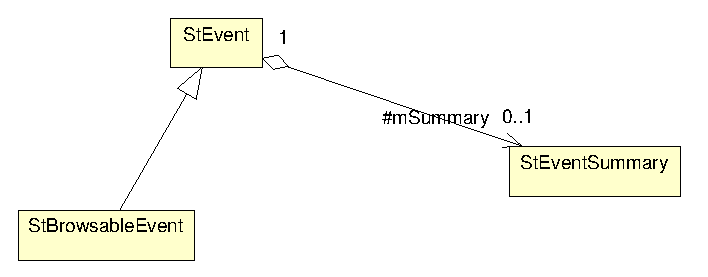
\includegraphics{event.eps}
        \caption{Class diagrams for \texttt{StEvent} and
            \texttt{StEventSummary}.}
    if (!tpcMon) return;       // no monitor 
    \end{center}
\end{figure}
The class \texttt{StEventSummary} contains lots of information
gathered during the reconstruction of the event like: the total number
of tracks, the number of positive or negative tracks, the number of
vertices of certain types, and several \emph{quasi}-histograms which
hold for example transverse momenta distributions and other important
quantities. The same warning as for \texttt{StRun} applies here.
Check the pointer to the event summary before you use it. It could be
\texttt{NULL}.
 
As already mentioned \texttt{StEvent} opens the door to all the info
there is on the DST.  In order to get there you have to navigate
through the tree. Only few objects, mostly container and collections,
can be reached directly from the \texttt{StEvent} objects.  Here's a
Here we are actually talking about two different things. The 
trigger and the trigger detectors. The trigger is put together from data 
recorded by a bunch of trigger detectors combined in some logic. So far STAR deals
with 3 levels of trigger numbered 0 -- 3.  Currently the only one
implemented is level-0 (L0). Others will follow.  All trigger classes
inherit from a common base class \texttt{StTrigger}. As mentioned
above, at the moment there is  only one derived class \texttt{StL0Trigger}
as depicted in Fig.~\ref{fig:umlTrigger}.
\item Primary vertices (mostly only one)
\item List of all V0 vertex candidates
\item List of all Xi vertex candidates
\item List of all kink vertex candidates
\item Level-0 trigger
\end{enumerate}
And remember, an object you get \emph{by pointer} is not guaranteed to
exist, an object you get \emph{by reference} always exist.
The class contains everything there is available about the actual trigger:
trigger word, trigger action word, multiplicities, and more. The trigger
is directly contained in the \texttt{StEvent} class. In order to get a pointer
to the L0 trigger use: \texttt{StEvent::l0Trigger()}. Even if we repeat
us here: it is a pointer and therefore can be \texttt{NULL}. At the moment
all simulations have no trigger data. You were warned.
\index{software monitors}
The trigger detectors are those detectors which data is used in
the trigger (which doesn't mean that the data isn't useful for other
things as well). There's a couple of them: the Central Trigger Barrel
(CTB), the Zero Degree Calorimeter (ADC), the Vertex Position Detector
(VPD), and the Multiwire Proportional Chamber (MWC). This means we need
a collection to hold them together and indeed this is what
\texttt{StTriggerDetectorCollection}
is all about. The trigger detector design is shown in Fig.~\ref{fig:umlTrigger}.
The collection holds all classes which describe the different trigger detectors:
\texttt{StMwcTriggerDetector}, \texttt{StCtbTriggerDetector}, \texttt{StZdcTriggerDetector}, and
\texttt{StVpdTriggerDetector} (not shown). 
These trigger detectors store the actual ADC and TDC values including some
calculated quantities. Check in the reference section for more details.
The collection is a member of \texttt{StEvent}. To get a pointer to the
collection use: \texttt{StEvent::triggerDetectorCollection()}. From there you get the
specific trigger detectors through a set of methods.
The methods are named after the component they return by \texttt{reference}:
\texttt{ctb()} returns a reference to the \texttt{StCtbTriggerDetector},
\texttt{mwc()} to the \texttt{StMwcTriggerDetector}, and so on.
Since they are returned by reference you can be sure the objects exist. No checks
necessary. Note that ``exist'' is not a synonym for ``makes sense''. The reason
for this is that the DST contains the data for all trigger detectors in one big
table. If it available the collection (StTriggerDetectorCollection) is created
else \texttt{StEvent::triggerDetectorCollection()} will return \texttt{NULL}.
Once created the data in the table is used to setup the instances of the
various trigger detectors. If a specific detector wasn't used its data is set 0
(so the author hopes) but the data is still there. 
\texttt{StTpcSoftwareMonitor}, \texttt{svt()} to the
\texttt{StSvtSoftwareMonitor} -- well, you get the idea. As usual you
should check for \texttt{NULL} pointers. If a detector was not
reconstructed in the reconstruction chain it's likely that you will
not find the corresponding monitor.

The specific software monitor classes are pretty simple flat classes.
They have no relation with any other class. All they do is to hold
data. Because of this, they have no member access functions and all
data members are public. In order to make things easier for people
moving from table-based analysis to \StEvent-based analysis we kept
even the table names.  With other words the software monitor classes
match their table counterparts 1:1.  The names are not always
descriptive but the author got tired of inventing new names.  You'll
find more details on what is what in the reference section of this
             << ctb.time(i) << endl; 

Here a simple example on how to use the software monitors:
\begin{verbatim}
void printTpcClusterInfo(ostream& os = cout, StEvent* event)
{
    StTpcSofwareMonitor *tpcMon = 0;

    if (event && event->softwareMonitor())
        tpcMon = event->softwareMonitor()->tpc();
    else 

    if (!tpcMon) return;       // no monitor

Again, we are using the \texttt{PR()} macro from \texttt{StGlobals.hh} to save
some typing. The names of the method say all there is to say.
        os << "Inner sector " << i << " has "
           << tpcMon->n_clus_tpc_in[i] << " cluster" << endl;
\index{tracks} This is probably the most complex part of the design.
Before we go into the details we give a brief introduction to what a
track is and explain the differences between \emph{global} and
\emph{primary} tracks. We then introduce the track \emph{node}, which
plays a very central role in the \StEvent\ track model.  The different
blocks of information which make a track such as the track geometry
and the various traits are explained later together with a short
introduction to filters which, as you will learn, allow to apply
predefined algorithm to select and filter information out of the data.

The \textbf{trigger} is put together from data recorded by a bunch of
\index{primary tracks} \index{global tracks} The STAR tracker, known
as \texttt{tpt}, performs the tracking in the main STAR tracking
detector the TPC. It finds a set of hits, which tpt assume to belong
to one track and applies fits in order to determine the track
parameters. Once this is done the track is passed along the chain.
Points from other detectors might be added. At the end this track is
then usually fitted with a more sophisticated fitting method and from
there on is called a \textbf{global} track (class
        \caption{Class diagrams for the trigger detector collection and
            the \texttt{StTrigger} hierarchy.}
    cout << "  counter  |     mips    |     time   \n";
    cout << "--------------------------------------\n";
simulations have no trigger data. You were warned.
this, since by using all global tracks we can deduce the primary
vertex (or vertices) with pretty good accuracy. A track which comes
from the primary vertex (and most do) can be re-fitted using the new
primary vertex. This increase dramatically the accuracy in which STAR
can measure particles, both in terms of direction and momentum. If a
global track points back close enough to the primary vertex and the
re-fitting works out well (whatever that means) then this track, or
better the refitted track, becomes a \textbf{primary} track (class
\texttt{StPrimaryTrack}). A primary track only makes sense if it
refers to a primary vertex.  If a primary track is found the global
track which was used to create it makes almost no sense any more and
could be dropped, \texttt{if} you trust the procedure. However, things
aren't as perfect and a primary track very well could have been
misidentified.  For that reason STAR keeps currently all global
holds all classes which describe the different trigger detectors:
\texttt{StMwcTriggerDetector}, \texttt{StCtbTriggerDetector},
\texttt{StZdcTriggerDetector}, and \texttt{StVpdTriggerDetector} (not
shown).  These trigger detectors store the actual ADC and TDC values
a fraction of the global tracks if th primary track is superior. \\
If a primary track fit succeeds the new track parameters and related
get a pointer to the collection use:
the number of hits might change, since the newly re-fitted track might
exclude old hits and/or add new hits.  \StEvent\ is able to cope with
named after the component they return by reference: \texttt{ctb()}
returns a reference to the \texttt{StCtbTriggerDetector},
\texttt{mwc()} to the \texttt{StMwcTriggerDetector}, and so on.  Since
So far so good. But what is with the tracks which fail the fit.
checks necessary. Note that ``exist'' is not a synonym for ``makes
sense''. The reason for this is that the DST contains the data for all
trigger detectors in one big table. If it available the collection
(StTriggerDetectorCollection) is created else
\texttt{StEvent::triggerDetectorCollection()} will return
\texttt{NULL}.  Once created the data in the table is used to setup
the instances of the various trigger detectors. If a specific detector
wasn't used its data is set 0 (so the author hopes) but the data is
still there.

Here's an example which dumps the CTB data in form of a table:
\begin{verbatim}
void dumpCtb(StEvent* event)
{
not know a priori or at least cannot be determined unabmigiously. In

    StCtbTriggerDetector &ctb = event->triggerDetectorCollection()->ctb();
possibly also the set of hits used.  In a sense these are tracks
created from the same \texttt{seed}. How we keep track of all these
different flavours is explained in the next section.

    for (int i=0; i<ctb.numberOfTrays(); i++) 
        for (int j=0; j<ctb.numberOfSlats(); j++) 
            cout << setw(5) << i <<   " | "
used to re-fit the primary tracks.
                 << setw(10) << ctb.mips(i, j, 0) << " | "
                 << ctb.time(i, j, 0) << endl;
\index{track node}
As we have seen in the previous section there are two kinds of tracks
from which each of them might be possibly fitted in different models
such creating a whole bunch of tracks which all come originally from
the same \texttt{seed} formed early in the reconstruction chain. Only
one of them can be right (at least for a specific analysis) and if we
count tracks we can only count all of them as one. May students spent
by far too much time hunting
the problem of double-counting.\\
\end{verbatim}
Again, we are using the \texttt{PR()} macro from \texttt{StGlobals.hh}
to save some typing. The names of the methods speak for themself.
        \caption{Schematic view of the track node collection and its relation to
            the detector info collection and the list of daughter
            tracks of the primary vertex.}

This is probably the most complex part of the design.  Before we get
into too much detail we give a brief introduction on what a track is
We have to have a way to tell that all these flavours belong together
even if the have different fit parameters or event a slightly
different set of hits. This is were the track \textbf{node} comes into
the game (class \texttt{StTrackNode}).
various traits are explained later together with a short introduction
to filters, which, as you will learn, allow to apply predefined
Every track knows about the node it belongs and thus one can navigate
from one track in the node to the other.  Each node contains at 1--n
tracks. This is depicted in Fig.~\ref{fig:nodes}.

The array shown in the middle of the picture shows the list of nodes
as held by the StEvent class itself. Every element (depicted as a box)
The STAR tracker, known as \texttt{tpt}, performs the tracking in the
main STAR tracking detector the TPC. It finds a set of hits, which
between: max(N$_{primary}$, N$_{global}$) and N$_{primary}$ + N$_{global}$.
It is a good measure for the multiplicity in the event. 
passed along the chain.  Points from other detectors might be added.
At the end this track is then fitted with a more sophisticated fitting
primary vertex can be found easily secondary vertices are more tricky
to detect (at least in a Heavy-Ion collision) and can hardly be
identified unambiguously. If one could do so, one could repeat the
\subsubsection{Track Geometry and Fit Traits}

\subsubsection{PID Traits}

To summarize: STAR has two kinds of tracks global tracks which can
come from wherever they want and primary tracks which always point
back to the primary vertex. The position of the primary vertex was
        \caption{}
\label{sec:node}
\index{track node}

\vfill

       // Assume it's a pion
cout << tpcDedx.traits()->mean() << endl;
     << theHits.size() << " hits" << endl;

for (int i=0; i<theHits.size(); i++) {
    cout << theHits[i]->position() << endl;
%    Reference Manuel
    assert(theHits[i]->ladder() == iladder);
    assert(theHits[i]->wafer() == iwafer);
\part{Reference Manuel}
\end{verbatim}

\subsection{Remarks on Hits and Vertices}
\index{StMeasuredPoint}
The fact that hits and vertices inherit from the same base class
\texttt{StMeasuredPoint} can be used wherever positions and errors
are what count. Take for an example a track fit. What you have to pass
to the fitting algorithm are the points and the errors. A fitter usually
gives a damn if the position was taken in the SVT or TPC. What counts
are the coordinates and their weight which depends on the errors.
\end{verbatim}
In general each class
has a public:
as argument, extract the points and the vertex, and fills them in a vector.
It doesn't matter if the track is a global or a primary track or where ever
the hits may come from. This could look as follows:
\item Assignement operator
void fillPoints(vector<StMeasuredPoint*> vec, StTrack *track)
{
There are a few exceptions from this rule which are explained
in the referring class reference.
    //
    //   First add hits
trivial and their names are chosen such that one can easily figure out what
they are all about.
Macros and \texttt{Inline} declarations are omitted
throughout the documentation and so is the \texttt{virtual} keyword.
The state-of-the-art reference is always the class definition in the header
file.
\clearpage

  //
  // Get the StRichCollection
  // 
  StRichCollection* theRichCollection = mEvent->richCollection();
\item[Summary]
    Version of  \texttt{StEvent} with a higher degree of integration in ROOT.
    cout << "Aborting...\n" << endl;
    return kStWarn;
  }
\item[Description]
    \texttt{StBrowsableEvent} adds ROOT specific
  //
  // Get the Hits from the collection
  //
  if (!theRichCollection->hitsPresent()) {
\item[Related Classes]
    \texttt{StBrowsableEvent} is derived from \texttt{StEvent}.
    return kStWarn;
  }
  StSPtrVecRichHit& theRichHits = theRichCollection->getRichHits();

  //
  //
  StSPtrVecTrackNode& theTrackNodes = mEvent->trackNodes();
\end{verbatim}

\subsection{The L3 Trigger}
\index{L3Trigger}

The L3Trigger class looks in essence like the ``little brother'' of
the StEvent class. It provides a subset of the data member and methods
from StEvent with respect to TPC hits, track nodes and vertices.  This
allows, to some extend, to use exactly the same analysis code for the
\item[Summary]
    Definitions of all container types used in \StEvent.
standard offline reconstruction chain.
The only difference is that
\item[Description]
   \texttt{StContainers.h} includes \texttt{StArray.h} which contains the guts
    of the container implementation. In StContainer.h (and .cxx) the appropriate
    macros are called to declare and define the container types. If a new container
    type has to be defined it \emph{must} be defined here and only here.
\end{verbatim}
with
\begin{verbatim}
\subsection{StBrowsableEvent}
\index{StBrowsableEvent|textbf}
\label{sec:StBrowsableEvent}
\begin{Entry}
\item[Summary] Version of \texttt{StEvent} with a higher degree of
\item[Summary]
    Monitors details of the Central Trigger Barrel (CTB) reconstruction.
    \verb+#include "StBrowsableEvent.h"+\\
    \verb+class StBrowsableEvent;+\\
\item[Description] \texttt{StBrowsableEvent} adds ROOT specific
    features to \texttt{StEvent} such as to allow the navigation
    through \StEvent\ in a graphical data browser.
    \texttt{StEventMaker::event()} actually returns an instance of
    StBrowsableEvent not StEvent.
    \texttt{StEvent}.
\item[Public\\ Constructors]
    \verb+StBrowsableEvent();+\\

    \verb+StBrowsableEvent(const event_header_st&,+\\
    \verb+                 const dst_event_summary_st&,+\\
    \verb+                 const dst_summary_param_st&);+\\

    \verb+StBrowsableEvent(const event_header_st&);+\\
\item[Public Member\\ Functions]
    \verb+void browse(TBrowser*);+\\
\end{Entry}
\item[Summary]
    Central Trigger Barrel (CTB) data.

     StEvent* event;
     // ...
     event->l3Trigger()->someMethod();
\end{verbatim}
Only the entry point \texttt{event} has to be replaced by \texttt{event->l3trigger()}.
but can more complex ones as pointers to \texttt{StTrack} objects for example.
a pair to name just one of many applications. 

\clearpage
%%%%%%%%%%%%%%%%%%%%%%%%%%%%%%%%%%%%%%%%%%%%%%%%%%%%%%%%%%%%%%%%%%%%
%    Reference Manual
%%%%%%%%%%%%%%%%%%%%%%%%%%%%%%%%%%%%%%%%%%%%%%%%%%%%%%%%%%%%%%%%%%%%
\clearpage

\section{Class References} %%%%%%%%%%%%%%%%%%%%%%%%%%%%%%%%%%%%%%%%%
The classes which are currently implemented and available from the
STAR CVS repository are listed in alphabetic order.

Inherited member functions and operators are not described in the
reference section of a derived class. Always check the section(s) of
the base class(es) to get a complete overview on the available
methods.

In general each class has a public:
\begin{itemize}
\item Default constructor
\item Copy constructor
\item Assignment operator
\item Virtual destructor
\end{itemize}
There are a few exceptions from this rule which are explained in the
referring class reference.

Not every member function listed is explained in detail since many are
trivial and their names are chosen such that one can easily figure out
    \texttt{np}, dE/dx mean \texttt{dedx}, and sigma \texttt{sig}.
omitted throughout the documentation and so is the \texttt{virtual}
keyword.  The state-of-the-art reference is always the class
definition in the header file.
\begin{figure}[htb]
    \begin{center}
\item[Summary] Central Trigger Barrel (CTB) data.
            a common structure and a common behavior.}
    \end{center}
    \verb+Float_t sigma() const;+\\
    Returns the sigma of the dE/dx value.
\item[Summary] Definitions of all container types used in \StEvent.
    \verb+#include "StContainers.h"+\\
    \verb+UInt_t numberOfCtbCounters() const;+\\

    \verb+Float_t mips(UInt_t) const;+\\

    \verb+Float_t time(UInt_t) const;+\\

    \verb+void setMips(UInt_t, Float_t);+\\

    \verb+void setTime(UInt_t, Float_t);+\\
    \verb+UInt_t numberOfSlats() const;+\\
    Returns number of slats (usually 2).
    \texttt{1-(1+npresamples+npostsamples-1)} are the other "events",
    in chronological order.  For example, assuming 3 pre events and 2
    
    \verb+UInt_t numberOfPostSamples() const;+\\
    \item[evt = 1] 1st pre event at t = -3
    \item[evt = 2] 2nd pre event at t = -2
    Total energy (or ADC sum) in EMC.  
    \item[evt = 4] 1st post event at t = +1
    \item[evt = 5] 2nd post event at t = +2
    \verb+StEmcModule();+\\
\item[Public Member\\ Functions]
    \verb+UInt_t numberOfHits() const;+\\
    \verb+StSPtrVecEmcRawHit& hits();+\\
    \verb+const StSPtrVecEmcRawHit& hits() const;+\\
\end{Entry}
\item[Summary]
    Header file which contains all enumeration types
    used in \StEvent.

\subsection{StEmcPoint}
\item[Description]
    All enumeration types used in \StEvent\ are defined
    in this header file. It also includes other header files
    which are common to all STAR code. For a complete list
    of enum types see section \ref{sec:Enumerations}.
\item[Synopsis]
    \verb+#include "StEmcPoint.h"+\\
    \verb+class StEmcPoint;+\\
\item[Description]
\item[Related Classes]
\item[Public\\ Constructors]
    \verb+StEmcPoint();+\\
    \verb+StEmcPoint(const StThreeVectorF&,+\\
\item[Summary]
    Event header and entry point to the \StEvent\ tree.
    \verb+const StThreeVectorF&,+\\
    \verb+ULong_t, Float_t,+\\
    \verb+Float_t, Float_t,+\\
\item[Description]
    The class \texttt{StEvent} is the key class to work with
    the whole \StEvent\ tree. It itself contains data which
    describes and characterizes the event and gives
    references and pointers to all information there is in the event.
    Don't forget to check for \texttt{NULL} pointers if a method returns
    an object by pointer. Only if a method returns an object by reference
    \verb+StThreeVectorF size() const;+\\
    The package StEventMaker (see Sec.~\ref{sec:StEventMaker}) provides
    a pointer to the current instance of \texttt{StEvent}.
\item[Related Classes]
    Class \texttt{StEvent} inherits from \texttt{St\_DataSet}.
    \texttt{StBrowsableEvent} is derived from \texttt{StEvent}.
    \verb+StPtrVecEmcCluster& cluster(const StDetectorId);+\\
    \verb+const StPtrVecEmcCluster& cluster(const StDetectorId) const;+\\
    \verb+StPtrVecEmcPoint& neighbor();+\\
    \verb+const StPtrVecEmcPoint& neighbor() const;+\\
    \verb+void addNeighbor(const StEmcPoint*);+\\
    \verb+StPtrVecTrack& track();+\\
    \verb+const StPtrVecTrack& track() const;+\\
    \verb+void addTrack(StTrack*);+\\
\end{Entry}
\clearpage


    Character string which contains a short description
    of the type of the event you got.
\label{sec:StEmcRawHit}
\begin{Entry}
\item[Summary]
\item[Synopsis]
    \verb+#include "StEmcRawHit.h"+\\
    \verb+class StEmcRawHit;+\\
\item[Description]
\item[Related Classes]
\item[Public\\ Constructors]
    \verb+StEmcRawHit();+\\
    \verb+StEmcRawHit(StDetectorId, UInt_t, UInt_t, UInt_t, UInt_t);+\\
    \verb+ULong_t bunchCrossingNumber() const;+\\
    \verb+StDetectorId detector() const;+\\
    \verb+UInt_t module() const;+\\
    \verb+UInt_t eta() const;+\\
    Returns pointer to the event summary with many useful
    information for QA/QC and event characterization.
    \verb+Float_t energy() const;+\\
    \verb+void setId(StDetectorId, UInt_t, UInt_t, UInt_t);+\\
    \verb+void setAdc(const UInt_t);+\\
    \verb+void setEnergy(const Float_t);+\\
\end{Entry}
    gathered during the event reconstruction. Mostly statistic
    on number of hits, tracks etc.

\subsection{StEmcSoftwareMonitor}
    \texttt{St\_DataSet}.  \texttt{StBrowsableEvent} is derived from
    Pointer to the TPC hit collection. If no hits are stored
    on the DST this pointer is \texttt{NULL}. You better check for this.
\begin{Entry}
\item[Summary]
\item[Synopsis]
    Pointer to the FTPC hit collection. If no hits are stored
    on the DST this pointer is \texttt{NULL}. You better check for this.
\item[Description]
\item[Related Classes]
\item[Public\\ Constructors]
    Pointer to the SVT hit collection. If no hits are stored
    on the DST this pointer is \texttt{NULL}. You better check for this.
\clearpage
\begin{Entry}
\item[Summary] Header file which contains all enumeration types used
    in \StEvent.
\item[Synopsis]
    \verb+#include "StEnumerations.h"+\\
\item[Description] All enumeration types used in \StEvent\ are defined
    in this header file. It also includes other header files which are
    common to all STAR code. For a complete list of enum types see
    section \ref{sec:Enumerations}.
\end{Entry}
\clearpage


\subsection{StEvent}
\index{StEvent|textbf}
    Number of primary vertices (aka event vertices).
    Usually there is only one but future implementations of the
    vertex finder will be able to also detect pile-up vertices
    in which case you better check the number before dealing
    with the event.
    \verb+#include "StEvent.h"+\\
    \verb+class StEvent;+\\
\item[Description] The class \texttt{StEvent} is the key class to work
    with the whole \StEvent\ tree. It itself contains data which
    describes and characterizes the event and gives references and
    pointers to all information there is in the event.  Don't forget
    to check for \texttt{NULL} pointers if a method returns an object
    by pointer. Only if a method returns an object by reference
    it is guaranteed to exist.\\
    The package StEventMaker (see Sec.~\ref{sec:StEventMaker})
    provides a pointer to the current instance of \texttt{StEvent}.
\item[Related Classes] Class \texttt{StEvent} inherits from
    \texttt{St\_DataSet}.
\item[Public\\ Constructors]

    
    \verb+StEvent(const event_header_st&,+\\
    defaults to the first (\texttt{i=0}).
    Overwrite inherited \texttt{Browse()} method from \texttt{St\_DataSet}.
    Method is invoked from ROOT to allow interactive browsing of \StEvent. 
    
    \verb+Long_t runId() const;+\\
    Unique run identifier.
    
    \verb+Long_t time() const;+\\
    Time when the event was taken.
    
    \verb+ULong_t triggerMask() const;+\\

    \verb+ULong_t bunchCrossingNumber(Uint_t i) const;+\\       
    Returns the bunch crossing numbers, i.e.~two 32 bit words.
    \texttt{i = 0} returns the lower and \texttt{i = 1} the upper number.
    \verb+StEmcCollection* emcCollection();+\\

    \verb+const StRichCollection* richCollection() const;+\\
    \verb+const StEventInfo* info() const;+\\
    \texttt{StEventInfo} provides no additional information but is solely
    StEvent. See also \ref{sec:StEventInfo}.

    \verb+const StSoftwareMonitor* softwareMonitor() const;+\\
    holds ``monitors'' for every detector which contain information
    number of hits, tracks etc.
    \verb+StTpcHitCollection* tpcHitCollection();+\\
    Pointer to the TPC hit collection. If no hits are stored on the
    Pointer to the FTPC hit collection. If no hits are stored on the
    DST this pointer is \texttt{NULL}. You better check for this.

    \verb+StSvtHitCollection* svtHitCollection();+\\
    \verb+const StSvtHitCollection* svtHitCollection() const;+\\
    Pointer to the SVT hit collection. If no hits are stored on the
    DST this pointer is \texttt{NULL}. You better check for this.    

    \verb+StSsdHitCollection* ssdHitCollection();+\\
    \verb+const StSsdHitCollection* ssdHitCollection() const;+\\
    Pointer to the SSD hit collection. If no hits are stored on the
    DST this pointer is \texttt{NULL}. You better check for this.   

    \verb+StL0Trigger* l0Trigger();+\\
    \verb+const StL0Trigger* l0Trigger() const;+\\

    \verb+StL3Trigger* l3Trigger();+\\
    \verb+const StL3Trigger* l3Trigger() const;+\\

    Returns pointer to the current trigger detector collection.
    Trigger detectors are CTB, ZDC, VPD, and MWC.
    
    \verb+StSPtrVecTrackDetectorInfo& trackDetectorInfo();+\\
    \verb+const StSPtrVecTrackDetectorInfo& trackDetectorInfo() const;+\\
    
    \verb+StSPtrVecTrackNode& trackNodes();+\\
    \verb+const StSPtrVecTrackNode& trackNodes() const;+\\
    
    \verb+UInt_t numberOfPrimaryVertices() const;+\\
    Number of primary vertices (aka event vertices).  Usually there is
    check the number before dealing with the event.
    \verb+void setSummary(StEventSummary*);+\\
    

    \verb+void setEmcCollection(StEmcCollection*);+\\

    \verb+void setRichCollection(StRichCollection*);+\\

    the vertex with the most daughter tracks.\index{primary vertices, order of}
    
    \verb+StSPtrVecXiVertex& xiVertices();+\\
    \verb+const StSPtrVecXiVertex& xiVertices() const;+\\
    Returns container with Xi vertices.
    
    \verb+StSPtrVecKinkVertex& kinkVertices();+\\
    \verb+const StSPtrVecKinkVertex& kinkVertices() const;+\\
    \verb+void setBunchCrossingNumber(ULong_t);+\\
    
    \verb+void setType(const Char_t*);+\\

    \verb+void setRunId(Long_t);+\\

    \verb+void setId(Long_t);+\\

    \verb+void setTime(Long_t);+\\

\item[Summary]
    Header files which contains all type definition used in \StEvent.
    \verb+void setBunchCrossingNumber(ULong_t, UInt_t);+\\

\item[Description]
    Since all \StEvent\ classes contain only the minimum amount of declaration
    it could become very tedious to find the right set of header files in your application.
    This header files overcomes this problem. Include it and you are all set.
    See also section \ref{sec:HeaderFiles}.
    \verb+ULong_t bunchCrossingNumber() const;+\\
    \verb+StEventInfo(const event_header_st&);+\\
\item[Public Member\\ Functions]
    \verb+const TString& type() const;+\\
    \verb+Long_t id() const;+\\
    \verb+Long_t runId() const;+\\
    \verb+void setBunchCrossingNumber(ULong_t);+\\
    \verb+ULong_t triggerMask() const;+\\

    \verb+ULong_t bunchCrossingNumber(Uint_t i) const;+\\
    Returns the bunch crossing numbers, i.e.~two 32 bit words.
    \texttt{i = 0} returns the lower and \texttt{i = 1} the upper number.

    \verb+static bool removeTriggerDetectorCollection(StEvent*);+\\
    \verb+static bool removeL3Trigger(StEvent*);+\\
    \verb+static bool removeV0Vertices(StEvent*);+\\
    Do not remove the TPC hits via \texttt{removeTpcHitCollection()}
    if you use this method.
\end{Entry}

\subsection{StEventSummary}
\index{StEventSummary|textbf}
    Returns sector number running from 0--5.

\item[Summary]
    Returns plane number running from 0--19.
    \verb+#include "StEventSummary.h"+\\
    \verb+ULong_t padsInCluster() const;+\\
    \verb+ULong_t timebinsInCluster() const;+\\
\item[Related Classes]
\item[Public\\ Constructors]
    \verb+StEventSummary();+\\
    \verb+StEventSummary(const dst_event_summary_st&,+\\
    \verb+               const dst_summary_param_st&);+\\
\item[Public Member\\ Functions]
    \verb+Long_t numberOfTracks() const;+\\
    \verb+Long_t numberOfGoodTracks() const;+\\
    \verb+Long_t numberOfGoodTracks(StChargeSign) const;+\\
    \verb+Long_t numberOfGoodPrimaryTracks() const;+\\
    \verb+Long_t numberOfExoticTracks() const;+\\
    \verb+Long_t numberOfVertices() const;+\\
    \verb+Long_t numberOfVerticesOfType(StVertexId) const;+\\
    \verb+Long_t numberOfPileupVertices() const;+\\
    \verb+Float_t meanPt() const;+\\
    \verb+Float_t meanPt2() const;+\\
    \verb+Float_t meanEta() const;+\\
    \verb+Float_t rmsEta() const;+\\
    \verb+const StThreeVectorF& primaryVertexPosition() const;+\\
    \verb+UInt_t numberOfBins() const;+\\
    \verb+Long_t tracksInEtaBin(UInt_t) const;+\\
    \verb+Long_t tracksInPhiBin(UInt_t) const;+\\
    \verb+Long_t tracksInPtBin(UInt_t) const;+\\
    \verb+Float_t energyInEtaBin(UInt_t) const;+\\
    \verb+Float_t energyInPhiBin(UInt_t) const;+\\
    \verb+Float_t lowerEdgeEtaBin(UInt_t) const;+\\
    Index \texttt{i} runs from 0--(n-1) where n = \texttt{numberOfPlanes()}.
    \verb+Float_t upperEdgePhiBin(UInt_t) const;+\\
    \verb+Float_t lowerEdgePtBin(UInt_t) const;+\\
    \verb+Float_t upperEdgePtBin(UInt_t) const;+\\

    \verb+Double_t magneticField() const;+\\
    Returns z-component of magnetic field in kGauss.
    
    \verb+void setNumberOfTracks(Long_t);+\\
    \verb+void setNumberOfGoodTracks(Long_t);+\\

    \verb+void setNumberOfGoodPrimaryTracks(Long_t);+\\
    \verb+void setNumberOfNegativeTracks(Long_t);+\\
    \verb+void setNumberOfExoticTracks(Long_t);+\\
    \verb+void setNumberOfVertices(Long_t);+\\
    \verb+void setNumberOfVerticesForType(StVertexId, Long_t);+\\
\item[Related Classes]
   Instance of \texttt{StFtpcPlaneHitCollection} are stored in the \texttt{StFtpcHitCollection}.
   The class holds a list of objects of type \texttt{StFtpcSectorHitCollection}.
    \verb+void setMeanEta(Float_t);+\\
    \verb+void setRmsEta(Float_t);+\\
    \verb+void setPrimaryVertexPosition(const StThreeVectorF&);+\\
    \verb+void setMagneticField(Double_t);+\\
\end{Entry}
\clearpage


\subsection{StEventTypes}
\index{StEventTypes|textbf}
\label{sec:StEventTypes}
\begin{Entry}
\item[Summary] Header files which contains all type definition used in
    \StEvent.
    Returns the \texttt{i}'th sector, where \texttt{i = 0--(numberOfSectors()-1).}
\item[Description] Since all \StEvent\ classes contain only the
    minimum amount of declaration it could become very tedious to find
    the right set of header files in your application.  This header
    files overcomes this problem. Include it and you are all set.  See
    also section \ref{sec:HeaderFiles}.
\end{Entry}
\clearpage


\subsection{StFtpcHit}
\index{StFtpcHit|textbf}
\label{sec:StFtpcHit}
\begin{Entry}
\item[Summary]
\item[Synopsis]
    \verb+#include "StFtpcHit.h"+\\
    \verb+class StFtpcHit;+\\
\item[Description]
\item[Public\\ Constructors]
    \verb+StFtpcHit();+\\

    \verb+StFtpcHit(const StThreeVectorF&,+\\
    \verb+          const StThreeVectorF&,+\\
    \verb+          ULong_t, Float_t, UChar_t = 0);+\\

    \verb+StFtpcHit(const dst_point_st&);+\\
\item[Public Member\\ Functions]
    \verb+ULong_t sector() const;+\\
    Returns sector number running from 1--6.
    
    \verb+ULong_t plane() const;+\\
    Returns plane number running from 1--20.      

    \verb+ULong_t padsInHit() const;+\\
    \verb+ULong_t timebinsInHit() const;+\\
\clearpage


\subsection{StFtpcHitCollection}
\index{StFtpcHitCollection|textbf}
\label{sec:StFtpcHitCollection}
\begin{Entry}
\item[Summary]
\item[Synopsis]
    \verb+#include "StFtpcHitCollection.h"+\\
    \verb+class StFtpcHitCollection;+\\
\item[Description]
\item[Related Classes]
\item[Public\\ Constructors]
    \verb+StFtpcHitCollection();+\\
\item[Public Member\\ Functions]
    \verb+Bool_t addHit(StFtpcHit*);+\\
    
    \verb+ULong_t numberOfHits() const;+\\
    Total number of FTPC hits stored in the collection.
    
    \verb+UInt_t numberOfPlanes() const;+\\
    
    \verb+StFtpcPlaneHitCollection* plane(UInt_t i);+\\
    \verb+const StFtpcPlaneHitCollection* plane(UInt_t i) const;+\\
    Index \texttt{i} runs from 0--(n-1) where n =
\end{Entry}                            
\end{Entry}
\clearpage


\subsection{StFtpcPlaneHitCollection}
\index{StFtpcPlaneHitCollection|textbf}
\label{sec:StFtpcPlaneHitCollection}
\begin{Entry}
\item[Summary]
    
\item[Synopsis]
    \verb+#include "StFtpcPlaneHitCollection.h"+\\
    \verb+class StFtpcPlaneHitCollection;+\\
\item[Description]
    
\item[Related Classes] Instance of \texttt{StFtpcPlaneHitCollection}
    are stored in the \texttt{StFtpcHitCollection}.  The class holds a
    list of objects of type \texttt{StFtpcSectorHitCollection}.
   
\item[Public\\ Constructors]
    \verb+StFtpcPlaneHitCollection();+\\
    Default constructor.
    
\item[Public Member\\ Functions]
    \verb+ULong_t numberOfHits() const;+\\
    Number of hits stored in this FTPC plane.
    
    \verb+UInt_t numberOfSectors() const;+\\
    Number of sectors in this FTPC plane.
    
    Total number of SVT-TPC tracks matched with
    tan(dip angle) $< 0$  $(\ge 0)$.
    Returns the \texttt{i}'th sector, where \texttt{i =
        0--(numberOfSectors()-1).}
    Number of tracks used in primary vertex fit. 
\clearpage

    Primary vertex covariance matrix. 
\subsection{StFtpcSectorHitCollection}
\index{StFtpcSectorHitCollection|textbf}
    Primary vertex $\chi^2$ of fit.     
\begin{Entry}
\item[Summary]
\item[Synopsis]
    \verb+#include "StFtpcSectorHitCollection.h"+\\
    \verb+class StFtpcSectorHitCollection;+\\
\item[Description]
\item[Related Classes]
\item[Public\\ Constructors]
    \verb+StFtpcSectorHitCollection();+\\
\item[Public Member\\ Functions]
    \verb+StSPtrVecFtpcHit& hits();+\\
    
    \verb+const StSPtrVecFtpcHit& hits() const;+\\
\item[Related Classes]
    \texttt{StGlobalTrack} is derived from \texttt{StTrack}. See also
    \texttt{StPrimaryTrack}.


\subsection{StFtpcSoftwareMonitor}
\index{StFtpcSoftwareMonitor|textbf}
\label{sec:StFtpcSoftwareMonitor}
\begin{Entry}
\item[Summary]
\item[Synopsis]
    \verb+#include "StFtpcSoftwareMonitor.h"+\\
    \verb+class StFtpcSoftwareMonitor;+\\
\item[Description]
\item[Related Classes]
\item[Public\\ Constructors]
    \verb+StFtpcSoftwareMonitor();+\\

    \verb+StFtpcSoftwareMonitor(const dst_mon_soft_ftpc_st&);+\\
\item[Public Data\\ Member]
    \verb+Long_t n_clus_ftpc[2];+\\
    Total number of clusters in FTPC, east/west.
    
    \verb+Long_t n_pts_ftpc[2];+\\
    Total number of space points in FTPC, east/west.
    
    
    \verb+Float_t chrg_ftpc_tot[2];+\\
    
    \verb+Float_t hit_frac_ftpc[2];+\\
    
    Average track length (cm) FTPC, east/west \\
    or average number of points assigned.
    \verb+Float_t res_pad_ftpc[2];+\\
    \verb+Float_t res_drf_ftpc[2];+\\
\clearpage
\subsection{StFunctional}
\begin{Entry}
    \verb+#include "StFunctional.h"+\\
\clearpage


\subsection{StGlobalSoftwareMonitor}
\index{StGlobalSoftwareMonitor|textbf}
\label{sec:StGlobalSoftwareMonitor}
\begin{Entry}
\item[Summary]
\item[Synopsis]
    \verb+#include "StGlobalSoftwareMonitor.h"+\\
    \verb+class StGlobalSoftwareMonitor;+\\
\item[Description]
\item[Related Classes]
\item[Public\\ Constructors]
\item[Related Classes]
    \texttt{StHit} is derived form \texttt{StMeasuredPoint}.
\item[Public Data\\ Member]
    \verb+Long_t n_trk_match[2];+\\
    Total number of SVT-TPC tracks matched with tan(dip angle) $< 0$
    $(\ge 0)$.

    \verb+Long_t prim_vrtx_ntrk;+\\
    Number of tracks used in primary vertex fit.

    \verb+Float_t prim_vrtx_cov[6];+\\
    Primary vertex covariance matrix.

    \verb+Float_t prim_vrtx_chisq;+\\
    Primary vertex $\chi^2$ of fit.
\end{Entry}
\clearpage


\subsection{StGlobalTrack}
\index{StGlobalTrack|textbf}
\label{sec:StGlobalTrack}
\item[Synopsis]
    \verb+class StGlobalTrack;+\\
\item[Description]
\item[Related Classes] \texttt{StGlobalTrack} is derived from
    \texttt{StTrack}. See also \texttt{StPrimaryTrack}.
    
\item[Public\\ Constructors]
    \verb+StGlobalTrack();+\\
    \verb+StGlobalTrack(const dst_track_st&);+\\
    \verb+StGlobalTrack(const StGlobalTrack&);+\\
    \verb+StGlobalTrack& operator=(const StGlobalTrack&);+\\
\item[Public Member\\ Functions]
    \verb+StTrackType type() const;+\\
    Returns always \texttt{global}.

    \verb+const StVertex* vertex() const;+\\
    Returns always \texttt{null}.
\end{Entry}
\clearpage


\subsection{StHelixModel}
\index{StHelixModel|textbf}
\label{sec:StHelixModel}
\begin{Entry}
\item[Summary]
\item[Synopsis]
    \verb+#include "StHelixModel.h"+\\
    \verb+class StHelixModel;+\\
\item[Description]
\item[Related Classes]
    Inherits directly from \texttt{StTrackGeometry}.
    
\item[Public\\ Constructors]
    \verb+StHelixModel();+\\
    
    \verb+StHelixModel(Short_t q, Float_t psi, Float_t c, Float_t dip,+\\
    \verb+             const StThreeVectorF& o, const StThreeVectorF& p);+\\
    
    \verb+StHelixModel(const dst_track_st&);+\\
    
\item[Public Member\\ Functions]
    \verb+StTrackModel model() const;+\\
\item[Summary]
    Charge in units of +e.
    
    \verb+Double_t curvature() const;+\\
    Curvature in cm$^{-1}$.
\item[Related Classes] \texttt{StHit} is derived form
    \texttt{StMeasuredPoint}.

    \verb+const StThreeVectorF& origin() const;+\\
    Origin in cm.
    
    \verb+const StThreeVectorF& momentum() const;+\\
    Momentum in GeV/c.
    \verb+StPhysicalHelixD helix() const;+\\
\end{Entry}
    \verb+UChar_t flag() const;+\\
    \verb+UChar_t trackReferenceCount() const;+\\
    \verb+StThreeVectorF positionError() const; // overwrite inherited+\\
    \verb+StMatrixF covariantMatrix() const; // overwrite inherited+\\
\item[Public\\ Constructors]
    \verb+StHit(const StThreeVectorF&,+\\
    \verb+      const StThreeVectorF&,+\\
    \verb+      ULong_t, Float_t, UChar_t = 0);+\\
    
    \verb+Float_t charge() const;+\\
    Total charge of hit.
    
    \verb+UInt_t flag() const;+\\
    Returns status flag.
    
    \verb+UInt_t usedInFit() const;+\\
    Returns flag providing info on if this hit was actually used in one
    of the various track fits.
    
    \verb+UInt_t trackReferenceCount() const;+\\
    Returns the number of tracks associated with that hit.
    
    \verb+StDetectorId detector() const;+\\

    \verb+StThreeVectorF positionError() const;+\\

    \verb+StMatrixF covariantMatrix() const;+\\
    Returns covariant matrix. In unknown (or not overwritten) simply fills
    the diagonal elements with the errors obtained via \texttt{positionError()}.
    
    \verb+void setCharge(Float_t);+\\
    \verb+void setFlag(UChar_t);+\\
    \verb+void setTrackReferenceCount(UChar_t);+\\
    \verb+void setHardwarePosition(ULong_t);+\\
    \verb+void setPositionError(const StThreeVectorF&);+\\
    \verb+StPtrVecTrack relatedTracks(const StSPtrVecTrackNode&, StTrackType);+\\
    
\item[Public Member\\ Operators]
    \verb+Int_t operator==(const StHit&) const;+\\
    \verb+Int_t operator!=(const StHit&) const;+\\
\end{Entry}
\clearpage


\subsection{StKinkVertex}
\index{StKinkVertex|textbf}
\label{sec:StKinkVertex}
\begin{Entry}
\item[Summary]
\item[Synopsis]
    \verb+#include "StKinkVertex.h"+\\
    \verb+class StKinkVertex;+\\
\item[Description]
\item[Related Classes]
\item[Public\\ Constructors]
    \verb+StKinkVertex();+\\
    \verb+StKinkVertex(const dst_vertex_st&, const dst_tkf_vertex_st&);+\\
\item[Public Member\\ Functions]
    \verb+StVertexId type() const;+\\
    \verb+UInt_t numberOfDaughters() const;+\\
    \verb+StTrack* daughter(UInt_t = 0);+\\
    \verb+const StTrack* daughter(UInt_t = 0) const;+\\
    \verb+StPtrVecTrack daughters(StTrackFilter&);+\\
    \verb+StParticleDefinition* pidParent() const;+\\
    \verb+StParticleDefinition* pidDaughter() const;+\\
    \verb+UShort_t geantIdParent() const;+\\
    \verb+UShort_t geantIdDaughter() const;+\\
    \verb+Float_t dcaParentDaughter() const;+\\
    \verb+Float_t dcaDaughterPrimaryVertex() const;+\\
    \verb+Float_t dcaParentPrimaryVertex() const;+\\
    \verb+Float_t hitDistanceParentDaughter() const;+\\
    \verb+Float_t hitDistanceParentVertex() const;+\\
    \verb+Float_t dE(UInt_t i) const;+\\
    \verb+Float_t decayAngle() const;+\\
    \verb+Float_t decayAngleCM() const;+\\
    \verb+const StThreeVectorF& parentMomentum() const;+\\
    \verb+StThreeVectorF& parentMomentum();+\\
    \verb+const StThreeVectorF& daughterMomentum() const;+\\
    \verb+StThreeVectorF& daughterMomentum();+\\
    \verb+void setGeantIdParent(UShort_t);+\\
    \verb+void setGeantIdDaughter(UShort_t);+\\
    \verb+void setDcaParentDaughter(Float_t);+\\
    \verb+void setDcaDaughterPrimaryVertex(Float_t);+\\
    \verb+void setDcaParentPrimaryVertex(Float_t);+\\
    \verb+void setHitDistanceParentDaughter(Float_t);+\\
    \verb+void setHitDistanceParentVertex(Float_t);+\\
    \verb+void setdE(UInt_t, Float_t);+\\
    \verb+void setDecayAngle(Float_t);+\\
    \verb+void setDecayAngleCM(Float_t);+\\
    \verb+void setParentMomentum(const StThreeVectorF&);+\\
    \verb+void setDaughterMomentum(const StThreeVectorF&);+\\
    \verb+void addDaughter(StTrack*);+\\
    \verb+void removeDaughter(StTrack*);+\\
\end{Entry}
\clearpage


\subsection{StL0Trigger}
\index{StL0Trigger|textbf}
\label{sec:StL0Trigger}
\begin{Entry}
\item[Summary]
\item[Synopsis]
    \verb+#include "StL0Trigger.h"+\\
    \verb+class StL0Trigger;+\\
\item[Description]
\item[Related Classes]
\item[Public\\ Constructors]
    \verb+StL0Trigger();+\\
    \verb+StL0Trigger(const dst_L0_Trigger_st&);+\\
\item[Public Member\\ Functions]
    \verb+UInt_t coarsePixelArraySize();+\\
    \verb+Long_t coarsePixelArray(UInt_t);+\\
    \verb+Long_t mwcCtbMultiplicity() const;+\\
    \verb+Long_t mwcCtbDipole() const;+\\
    \verb+Long_t mwcCtbTopology() const;+\\
    \verb+Long_t mwcCtbMoment() const;+\\
    
    \verb+Long_t nTotalHits ;+\\
    Total number of clusters in the event.
    
    \verb+Long_t nTotalTracks;+\\
    Total number of tracks found by the tracker.
    
    \verb+Long_t nTotalPrimaryTracks;+\\
    Number of primary tracks found by the tracker.
    
    \verb+Short_t processorId[24] ;+\\
    Processor where the sector was reconstructed.
    
    \verb+Float_t vertex[3][24];+\\
    xyz coordinates of the vertex used for track finding.
    
    \verb+Short_t id_param[24];+\\
    The parameter set used in the tracker.
    
    \verb+Long_t nHits[24];+\\
    Number of clusters in the sector.
    
    \verb+Long_t nTracks[24];+\\
    Number of tracks found by the tracker.
    
    \verb+Long_t nPrimaryTracks[24];+\\
    Number of primary tracks found by the tracker.
    
    \verb+Float_t cpuTime[24];+\\
    CPU time used by the tracker.
\end{Entry}
\clearpage


\subsection{StL3Trigger}
\index{StL3Trigger|textbf}
\label{sec:StL3Trigger}
\begin{Entry}
\item[Summary]
\item[Synopsis]
    \verb+#include "StL3Trigger.h"+\\
    \verb+class StL3Trigger;+\\
\item[Description]
\item[Related Classes]
\item[Public\\ Constructors]
    \verb+StL3Trigger();+\\
    \verb+const StTpcHitCollection* tpcHitCollection() const;+\\

    \verb+StSPtrVecTrackDetectorInfo& trackDetectorInfo();+\\

    \verb+const StSPtrVecTrackNode& trackNodes() const;+\\
    \verb+StPrimaryVertex* primaryVertex(UInt_t = 0);+\\
    \verb+const StPrimaryVertex* primaryVertex(UInt_t = 0) const;+\\

    \verb+void addPrimaryVertex(StPrimaryVertex*);+\\
    \verb+UInt_t numberOfMwcSectors() const;+\\
    \verb+Float_t mips(UInt_t) const;+\\
    \verb+void setMips(UInt_t, Float_t);+\\
    \verb+UInt_t numberOfSectors() const;+\\
    \verb+UInt_t numberOfSubSectors() const;+\\
    Number of MWC subsectors (usually 4).
    
    Number of pre-samples available.
    
    \verb+UInt_t numberOfPostSamples() const;+\\
    data are simple reserved (on request of Hank Crawford) for
    possible future use.  For the second argument (\texttt{evt}) see
    
    \verb+void setAux(UInt_t, UInt_t, Float_t);+\\
    \verb+void setNumberOfPreSamples(UInt_t);+\\
\end{Entry}

\subsection{StPrimaryTrack}
\index{StPrimaryTrack|textbf}
\item[Summary]
    \verb+#include "StPrimaryTrack.h"+\\
    \verb+class StPrimaryTrack;+\\
\item[Description]
\item[Related Classes]
\item[Public\\ Constructors]
    \verb+StPrimaryTrack();+\\
    \verb+StPrimaryTrack(const dst_track_st&);+\\
    \verb+StPrimaryTrack(const StPrimaryTrack&);+\\
    \verb+StPrimaryTrack& operator=(const StPrimaryTrack&);+\\
\item[Public Member\\ Functions]
    \verb+StTrackType type() const;+\\
    \verb+const StVertex* vertex() const;+\\
    Returns always \texttt{primary}.

    \verb+void setVertex(StVertex*);+\\
    Returns pointer to actual primary (event) vertex.
\end{Entry}
\clearpage


\subsection{StPrimaryVertex}
    \verb+StRichPixel(UShort_t pad, UShort_t adc);+\\
    \verb+StRichPixel(const dst_rch_pixel_st&);+\\
\label{sec:StPrimaryVertex}
    \verb+UShort_t module() const;+\\
    \verb+UShort_t channel() const;+\\
    \verb+UShort_t adc() const;+\\
\item[Public Member\\ Operators]
\begin{Entry}
\item[Summary]

\item[Related Classes]
    Inherits directly from \texttt{StVertex}.
    
    are the ADC value (11th bit indicates overflow).

    \verb+StRichMCPixel(ULong_t packedData,+\\
\item[Summary]
        Coded data of the pixel where the first 8 bits are the pad
    number, the second 8 bits are the row, and the next 11 bits
    are the ADC value (11th bit indicates overflow) as well as
\item[Description]
    Equality operator based on the packed data ONLY.

    \verb+Int_t operator!=(const StRichMCPixel&) const;+\\
    \verb+UShort_t contributions() const;+\\
    Adds information to the Monte Carlo list.



\subsection{StRichPixelCollection}
\index{StRichPixelCollection|textbf}
\label{sec:StRichPixelCollection}
\begin{Entry}
\item[Summary]
\item[Synopsis]
    \verb+#include "StRichPixelCollection.h"+\\
\item[Description]
    \verb+StRichPixelCollection();+\\
    \verb+StRichPixelCollection(dst_rch_pixel_st*, int);+\\
\item[Public Member\\ Functions]
    \verb+StRichPixel pixel(unsigned int) const; // return a pixel+\\
    \verb+unsigned int size() const; // STL size of container+\\
    \verb+unsigned int numberOfPixels() const;+\\
\end{Entry}
\clearpage

    \verb+Int_t operator==(const StRichPidTraits&) const;+\\
    \verb+const StSPtrVecRichPid getAllPids() const;+\\
\end{Entry}
\subsection{StRichPixel}
\begin{Entry}
\item[Related Classes]
\item[Public\\ Constructors]
    \verb+StRichPixel();+\\
    Empty constructor.
    \verb+StRichPixel(ULong_t packedData);+\\
    Specify the pixel utilizing the packed data where
    the first 8 bits are the pad
    number, the second 8 bits are the row, and the next 11 bits
    are the ADC value (11th bit indicates overflow).
\item[Public Member\\ Functions]
    \verb+Int_t operator==(const StRichPixel&) const;+\\
    Equality operator based on the coded data.

    \verb+Int_t operator!=(const StRichPixel&) const;+\\
    Complement of the equality operator.

    \verb+void setPackedData(ULong_t);+\\
\item[Public Data\\ Member]

    Total multiplicity (or ADC sum) in RICH.
    \verb+UShort_t pad() const;+\\
    Returns the pad number.

    \verb+UShort_t row() const;+\\

    \verb+UShort_t adc() const;+\\
    Returns the adc value.



    \verb+ULong_t reservedLong() const;+\\
    Reserved for future use.

    \verb+void setReservedLong(ULong_t);+\\
    Reserved for future use.
\end{Entry}
\clearpage

\subsection{StRichSoftwareMonitor}
\index{StRichSoftwareMonitor|textbf}
\label{sec:StRichSoftwareMonitor}
\begin{Entry}
\item[Summary]
    \verb+void setNumberOfTracksCrossing(Long_t);+\\
    \verb+void setNumberOfTracksPidCalculated(Long_t);+\\
\clearpage


    \verb+void setNumberOfTracksAbove1Gev(Long_t);+\\
    \verb+void setNumberOfHitsInRings(Long_t);+\\
    \verb+void setNumberOfRings(Long_t);+\\
    \verb+Long_t numberOfTracksCrossing() const;+\\
    \verb+Long_t numberOfTracksPidCalculated() const;+\\
    \verb+Long_t numberOfTracksAbove1Gev() const;+\\
    \verb+Long_t numberOfHitsInRings() const;+\\
    \verb+Long_t mult_rich_tot;+\\
\end{Entry}

\subsection{StRun}
\index{StRun|textbf}
\label{sec:StRun}
\begin{Entry}
\item[Summary]
\item[Synopsis]
    \verb+#include "StRun.h"+\\
    \verb+class StRun;+\\
\item[Description]
\item[Related Classes]
\item[Public\\ Constructors]
    \verb+StRun();+\\
    \verb+StRun(const run_header_st&, const dst_run_summary_st&);+\\
    \verb+StRun(const run_header_st&);+\\
\item[Public Member\\ Functions]
    \verb+Long_t id() const;+\\
    \verb+Long_t bfcId() const;+\\
    \verb+const TString& type() const;+\\
    \verb+Long_t triggerMask() const;+\\
    \verb+Double_t centerOfMassEnergy() const;+\\
    \verb+Short_t beamMassNumber(StBeamDirection) const;+\\
    \verb+Short_t beamCharge(StBeamDirection) const;+\\

    \verb+Double_t magneticField() const;+\\
    Returns z-component of magnetic field in kGauss.
    
    \verb+StRunSummary* summary();+\\
    \verb+const StRunSummary* summary() const;+\\
    \verb+static const TString& cvsTag();+\\
    \verb+void setId(Long_t);+\\
    \verb+void setBfcId(Long_t);+\\
    \verb+void setType(const Char_t*);+\\
    \verb+void setTriggerMask(Long_t);+\\
    \verb+void setCenterOfMassEnergy(Double_t);+\\
    \verb+void setBeamMassNumber(StBeamDirection, Short_t);+\\
    \verb+void setBeamCharge(StBeamDirection, Short_t);+\\
    \verb+void setSummary(StRunSummary*);+\\
    \verb+void setMagneticField(Double_t);+\\
\item[Public Member\\ Operator]
    \verb+Int_t operator==(const StRun&) const;+\\
    \verb+Int_t operator!=(const StRun&) const;+\\
\end{Entry}
\clearpage


\subsection{StRunSummary}
\index{StRunSummary|textbf}
\label{sec:StRunSummary}
\begin{Entry}
\item[Summary]
\item[Synopsis]
    \verb+#include "StRunSummary.h"+\\
    \verb+class StRunSummary;+\\
\item[Description]
\item[Related Classes]
\item[Public\\ Constructors]
    \verb+StRunSummary();+\\
    \verb+StRunSummary(const dst_run_summary_st&);+\\
\item[Public Member\\ Functions]
    \verb+         const StThreeVectorF&,+\\
    \verb+         ULong_t, Float_t, UChar_t = 0);+\\
    \verb+Long_t startTime() const;+\\
    \verb+Long_t stopTime() const;+\\
    \verb+ULong_t centralStripNSide() const;+\\
    Runs from 0--767.

    \verb+Float_t meanNumberOfVertices() const;+\\
    Runs from 0--767.

    \verb+Float_t rmsNumberOfVertices() const;+\\
    \verb+Float_t meanMultiplicity(StDetectorId) const;+\\
    \verb+ULong_t matchingQualityFactor() const;+\\
    \verb+Float_t rmsMultiplicity(StDetectorId) const;+\\
    \verb+void setNumberOfEvents(ULong_t);+\\
    \verb+void setNumberOfProcessedEvents(ULong_t);+\\
    \verb+void setFtpcSoftwareMonitor(StFtpcSoftwareMonitor*);+\\
    \verb+void setEmcSoftwareMonitor(StEmcSoftwareMonitor*);+\\
    \verb+void setRichSoftwareMonitor(StRichSoftwareMonitor*);+\\
    \verb+void setCtbSoftwareMonitor(StCtbSoftwareMonitor*);+\\
    \verb+void setGlobalSoftwareMonitor(StGlobalSoftwareMonitor*);+\\
    \verb+void setL3SoftwareMonitor(StL3SoftwareMonitor*);+\\
\end{Entry}
\clearpage


\subsection{StSsdHit}
\index{StSsdHit|textbf}
\label{sec:StSsdHit}
\begin{Entry}
\item[Summary]
\item[Synopsis]
    \verb+#include "StSsdHit.h"+\\
\end{Entry}
\clearpage
    Layer in which hit is located. Layer number runs
    from 0--5.
\subsection{StSsdHitCollection}
\index{StSsdHitCollection|textbf}
    Ladder number runs from 0--7.
\begin{Entry}
\item[Summary]
    Wafer number runs from 0--6.
    \verb+#include "StSsdHitCollection.h"+\\
    \verb+ULong_t barrel() const; // barrel=[0-2]+\\
    Barrel number runs from 0--2.
\item[Related Classes]
\item[Public\\ Constructors]
    \verb+StSsdHitCollection();+\\
\item[Public Member\\ Functions]
    \verb+Bool_t addHit(StSsdHit*);+\\
    \verb+ULong_t numberOfHits() const;+\\
    \verb+UInt_t numberOfLadders() const;+\\
    \verb+StSsdLadderHitCollection* ladder(UInt_t);+\\
    \verb+const StSsdLadderHitCollection* ladder(UInt_t) const;+\\
    Ladder number runs from 1--8.

\subsection{StSsdLadderHitCollection}
\index{StSsdLadderHitCollection|textbf}
\label{sec:StSsdLadderHitCollection}
\begin{Entry}
\item[Summary]
\item[Synopsis]
    \verb+#include "StSsdLadderHitCollection.h"+\\
    \verb+class StSsdLadderHitCollection;+\\
\item[Description]
\item[Related Classes]
\item[Public\\ Constructors]
    \verb+StSsdLadderHitCollection();+\\
\item[Public Member\\ Functions]
    \verb+ULong_t numberOfHits() const;+\\
    \verb+UInt_t numberOfWafers() const;+\\
    \verb+StSsdWaferHitCollection* wafer(UInt_t);+\\
    \verb+const StSsdWaferHitCollection* wafer(UInt_t) const;+\\
\end{Entry}
\clearpage

\subsection{StSsdWaferHitCollection}
\index{StSsdWaferHitCollection|textbf}
\label{sec:StSsdWaferHitCollection}
\begin{Entry}
\item[Synopsis]
    \verb+class StSsdWaferHitCollection;+\\
    \verb+UInt_t numberOfLayers() const;+\\
    \verb+StSvtLayerHitCollection* layer(UInt_t);+\\
    \verb+const StSvtLayerHitCollection* layer(UInt_t) const;+\\
    \verb+StSPtrVecSsdHit& hits();+\\
    \verb+const StSPtrVecSsdHit& hits() const;+\\
\end{Entry}
\clearpage

\subsection{StSvtBarrelHitCollection}
\index{StSvtBarrelHitCollection|textbf}
\label{sec:StSvtBarrelHitCollection}
\begin{Entry}
\item[Summary]
\item[Synopsis]
    \verb+#include "StSvtBarrelHitCollection.h"+\\
    \verb+class StSvtBarrelHitCollection;+\\
\item[Description]
\item[Related Classes]
\item[Public\\ Constructors]
    \verb+StSvtBarrelHitCollection();+\\
\item[Public Member\\ Functions]
    \verb+ULong_t numberOfHits() const;+\\
    \verb+UInt_t numberOfLadders() const;+\\
    \verb+StSvtLadderHitCollection* ladder(UInt_t);+\\
    \verb+void setLayerNumber(Int_t);+\\
    \verb+const StSvtLadderHitCollection* ladder(UInt_t) const;+\\
\end{Entry}
\clearpage

\subsection{StSvtLayerHitCollection}
\index{StSvtLayerHitCollection|textbf}
\label{sec:StSvtLayerHitCollection}
\begin{Entry}
\item[Summary]
\item[Synopsis]
    \verb+#include "StSvtLayerHitCollection.h"+\\
    \verb+class StSvtLayerHitCollection;+\\
\item[Description]
\item[Related Classes]
\item[Public\\ Constructors]
    \verb+StSvtLayerHitCollection();+\\
\item[Public Member\\ Functions]
    \verb+ULong_t numberOfHits() const;+\\
    \verb+UInt_t numberOfLadders() const;+\\
    \verb+StSvtLadderHitCollection* ladder(UInt_t);+\\
    \verb+const StSvtLadderHitCollection* ladder(UInt_t) const;+\\
    \verb+void setLayerNumber(Int_t);+\\
\end{Entry}
\clearpage



\subsection{StSvtHit}
\index{StSvtHit|textbf}
\label{sec:StSvtHit}
\begin{Entry}
\item[Summary]
\item[Synopsis]
    \verb+#include "StSvtHit.h"+\\
    \verb+class StSvtHit;+\\
    \verb+StSvtHit();+\\
    \verb+StSvtHit(const StThreeVectorF&,+\\
    \verb+         const StThreeVectorF&,+\\
    \verb+         ULong_t, Float_t, UChar_t = 0);+\\
    \verb+StSvtHit(const dst_point_st&);+\\
\item[Public Member\\ Functions]
    Total number clusters in each SVT layer.
    Layer in which hit is located. Layer number runs from 1--6.

    Total number of space points in each SVT layer.
    or  average chisq(1) of fit.
    \verb+ULong_t wafer() const;+\\
    Wafer number runs from 1--7.
    Total charge deposition in each SVT layer.
    or average chisq(2) of fit.     
    Barrel number runs from 1--3.
    Fraction of hits used in each SVT layer.
    \verb+ULong_t hybrid() const;+\\
\end{Entry}
\clearpage


\subsection{StSvtHitCollection}
\index{StSvtHitCollection|textbf}
\label{sec:StSvtHitCollection}
    
    
\begin{Entry}
\item[Summary]
\item[Synopsis]
    \verb+#include "StSvtHitCollection.h"+\\
    \verb+class StSvtHitCollection;+\\
\item[Description]
\item[Related Classes]
\item[Public\\ Constructors]
    \verb+StSvtHitCollection();+\\
\item[Public Member\\ Functions]

    \verb+Bool_t addHit(StSvtHit*);+\\

    \verb+ULong_t numberOfHits() const;+\\

    \verb+UInt_t numberOfBarrels() const;+\\
    
    \verb+StSvtBarrelHitCollection* barrel(UInt_t);+\\
    \verb+const StSvtBarrelHitCollection* barrel(UInt_t) const;+\\
\end{Entry}
\clearpage


\subsection{StSvtLadderHitCollection}
\index{StSvtLadderHitCollection|textbf}
\begin{Entry}
\item[Summary]
\item[Synopsis]
    \verb+#include "StSvtLadderHitCollection.h"+\\
    \verb+class StSvtLadderHitCollection;+\\
\item[Description]
\item[Related Classes]
\item[Public\\ Constructors]
\item[Summary]
    \verb+ULong_t numberOfHits() const;+\\
    \verb+UInt_t numberOfWafers() const;+\\
    \verb+StSvtWaferHitCollection* wafer(UInt_t);+\\
\item[Description]
\item[Related Classes]

\subsection{StSvtSoftwareMonitor}
\index{StSvtSoftwareMonitor|textbf}
\label{sec:StSvtSoftwareMonitor}
\begin{Entry}
    \verb+StSvtSoftwareMonitor(const dst_mon_soft_svt_st&);+\\
    \verb+Long_t n_clus_svt[4];+\\
    \verb+StTpcDedxPidAlgorithm();+\\
    
    Fraction of hits used in each SVT/SSD barrel/layer. 
    \verb+ULong_t sector() const; // 0-23+\\
    \verb+ULong_t padrow() const; // 0-44+\\
    \verb+ULong_t padsInCluster() const;+\\
    \verb+ULong_t pixelsInCluster() const;+\\
    \verb+Float_t res_drf_svt;+\\
    Average residuals, drift direction, SVT \\
    or average chisq(2) of fit.
\end{Entry}
\clearpage


\subsection{StSvtWaferHitCollection}
\index{StSvtWaferHitCollection|textbf}
\label{sec:StSvtWaferHitCollection}
\begin{Entry}
\item[Summary]
\item[Synopsis]
    \verb+#include "StSvtWaferHitCollection.h"+\\
    \verb+class StSvtWaferHitCollection;+\\
\item[Description]
\item[Related Classes]
\item[Public\\ Constructors]
    \verb+StSvtWaferHitCollection();+\\
\item[Public Member\\ Functions]
    \verb+StSPtrVecSvtHit& hits();+\\
    \verb+const StSPtrVecSvtHit& hits() const;+\\
\end{Entry}
\clearpage


    Index \texttt{i} runs from 0--(n-1) where n = \texttt{numberOfSectors()}.
\label{sec:StTpcDedxPidAlgorithm}
\begin{Entry}
\item[Summary] Functor which allows to obtain PID information
    derived from the dE/dx of the track in the TPC.
\item[Synopsis]
    \verb+#include "StTpcDedxPidAlgorithm.h"+\\
    \verb+class StTpcDedxPidAlgorithm;+\\
    
\item[Description] This is an example of an \texttt{StPidAlgorithm}.
    Please handle it as such.  The functor selects the first
    \texttt{StTrackPidTraits} it encounters that \textit{(i)} is
    derived from the TPC and \textit{(ii)} uses the method passed as
    an argument to the constructor. The various methods added to this
    class were implemented by Craig Ogilvie (MIT).  For a more general
    overview see \ref{sec:pidTraits} and \ref{sec:pidAlgorithm}.
    
\item[Related Classes]
    \texttt{StTpcDedxPidAlgorithm} inherits directly from
    \texttt{StPidAlgorithm}.
    
\item[Public\\ Constructors]
    \verb+StTpcDedxPidAlgorithm(StDedxMethod = kTruncatedMeanId);+\\
    Creates instances of \texttt{StTpcDedxPidAlgorithm}. The argument
    is the dE/dx method of your choice. The default is
    \texttt{kTruncatedMeanId}, i.e.~the \texttt{kTruncatedMeanId}
    method is selected in case you do not provide an argument.  See
    \ref{sec:Enumerations} for possible methods. Note that the
\item[Summary]
    even implemented.
    
\item[Public Member\\ Functions]
    \verb+StParticleDefinition* operator() (const StTrack&, const StSPtrVecTrackPidTraits&);+\\
    \verb+const StDedxPidTraits* traits() const;+\\
    \verb+double numberOfSigma(const StParticleDefinition*) const;+\\
    \verb+double meanPidFunction(const StParticleDefinition*) const;+\\
    \verb+double sigmaPidFunction(const StParticleDefinition*) const;+\\
\end{Entry}
\clearpage

\subsection{StTpcHit}
    \verb+UShort_t row() const;+\\
\item[Summary]
    \verb+class StTpcHit;+\\
\item[Description]
\item[Related Classes]
\item[Public\\ Constructors]
    \verb+StTpcHit();+\\
    Default constructor.
    
    \verb+StTpcHit(const StThreeVectorF&,+\\
    \verb+         const StThreeVectorF&,+\\
    \verb+         ULong_t, Float_t, UChar_t = 0);+\\
    
    \verb+StTpcHit(const dst_point_st&);+\\
    
\item[Public Member\\ Functions]
    \verb+ULong_t sector() const;+\\
    Returns sector number in the range 1--24.
    
    \verb+ULong_t padrow() const;+\\
    Returns padrow number in the range 1--45.

    \verb+ULong_t padsInHit() const;+\\
    
    \verb+ULong_t pixelsInHit() const;+\\

    \verb+StTpcPadrowHitCollection* padrow(UInt_t);+\\
\label{sec:StTpcHitCollection}
\item[Synopsis]
    \verb+#include "StTpcHitCollection.h"+\\
    \verb+class StTpcHitCollection;+\\
\item[Description]
\item[Related Classes]
\item[Public\\ Constructors]
    \verb+StTpcHitCollection();+\\
\item[Public Member\\ Functions]
    \verb+Bool_t addHit(StTpcHit*);+\\
    
    \verb+ULong_t numberOfHits() const;+\\
    Total number of TPC hits in the collection.
    
    \verb+UInt_t numberOfSectors() const;+\\

    \verb+StTpcSectorHitCollection* sector(UInt_t i);+\\
    \verb+const StTpcSectorHitCollection* sector(UInt_t i) const;+\\
    Index \texttt{i} runs from 0--(n-1) where n =
    \texttt{numberOfSectors()}.
\end{Entry}
\clearpage


\subsection{StTpcPadrowHitCollection}
\index{StTpcPadrowHitCollection|textbf}
\label{sec:StTpcPadrowHitCollection}
\begin{Entry}
\item[Summary] Holds all hits stored in a padrow.
\item[Synopsis]
    \verb+#include "StTpcPadrowHitCollection.h"+\\
    \verb+class StTpcPadrowHitCollection;+\\
\item[Description]
\item[Related Classes]
\item[Public\\ Constructors]
    \verb+StTpcPadrowHitCollection();+\\
\item[Public Member\\ Functions]
    \verb+StSPtrVecTpcHit& hits();+\\
    Total number of tracks in TPC, tan(dip angle) $< 0$  $(\ge 0)$.
\end{Entry}
\clearpage


\subsection{StTpcPixel}
\index{StTpcPixel|textbf}
\label{sec:StTpcPixel}
\begin{Entry}
\item[Summary] 
\item[Synopsis]
    \verb+#include "StTpcPixel.h"+\\
    \verb+class StTpcPixel;+\\
\item[Description]
\item[Related Classes]
\item[Public\\ Constructors]
    \verb+StTpcPixel();+\\
    \verb+StTpcPixel(UShort_t, ULong_t);+\\
    \verb+StTpcPixel(const dst_pixel_st&);+\\
\item[Public Member\\ Functions]
    \verb+UShort_t detector() const;+\\
    
    \verb+UShort_t sector() const;+\\
    Returns sector in the range 1--24.

    \verb+UShort_t padrow() const;+\\
    Returns padrow in the range 1--45.

    \verb+ULong_t pad() const;+\\
    \verb+ULong_t timebin() const;+\\
    \verb+ULong_t adc() const;+\\
\item[Public Member\\ Operator]
    \verb+Int_t operator==(const StTpcPixel&) const;+\\
    \verb+Int_t operator!=(const StTpcPixel&) const;+\\
\end{Entry}
\clearpage


\subsection{StTpcSectorHitCollection}
\index{StTpcSectorHitCollection|textbf}
\label{sec:StTpcSectorHitCollection}
\begin{Entry}
\item[Summary]
\item[Synopsis]
    \verb+#include "StTpcSectorHitCollection.h"+\\
\item[Public\\ Constructors]
    
    Returns padrow hit collection. Note that \texttt{i}=0--44.
\subsection{StTpcSoftwareMonitor}
    \verb+StTrackFindingMethod findingMethod() const;+\\
    \verb+StTrackQualityScheme qualityScheme() const;+\\
    Quality control flag (sort of). Most important: \texttt{flag()} $> 0$ good,
    the status of the refit and much more. For a detailed (and actual) description
    \verb+class StTpcSoftwareMonitor;+\\
    \begin{description}
    \verb+UShort_t numberOfPossiblePoints(StDetectorId) const;+\\
    \end{description} 
    If no refit is performed by \texttt{egr} then the return value of flag()
    is defined as follows: 

    where 
  
    \begin{description}
    \verb+const StPtrVecTrackPidTraits pidTraits(StDetectorId) const;+\\
    \item[-x03] Bad fit, too many fit iterations 
    \item[-x04] Bad Fit, too many outlier removal iterations 
    \item[-x06] Bad fit, outlier could not be identified 
    \item[-x10] Bad fit, not enough points to start 
    \end{description} 

       and a good track has\\ 
           \texttt{yy = ipass+10*int(what+1.0) }

     where \texttt{ipass} indicated which pass through the TPC tracking the track
     was identified on and what identifies which pass through the segment formation
     routines the track was formed   

     SVT only tracks:\\ 
     \texttt{sign(1,svt\_track.flag)*200.+svt\_track.flag}

     where
     \begin{verbatim}

     \end{verbatim}
    \verb+StTrack();+\\
     Matched SVT and TPC tracks:\\ 
     \texttt{svt\_track.flag*10+sign(1,tpc\_track.flag)*500+tpc\_track.flag}

     FTPC only tracks:
     \begin{description}
     \item[x01] good primary track 
     \item[x02] good v0 track 
     \end{description} 
     
     In all cases: 
     if $|q| \ne 1$ then flag() returns -1*(flag()+20)\\ 
     if $|1/p_\perp| \ge 999999$ then flag() returns -x99 
    \verb+StTrack(const dst_track_st&);+\\
    \verb+UShort_t numberOfPoints(StDetectorId) const;+\\
    
    \verb+const StVertex* vertex() const = 0;+\\
    Pointer to parent vertex.
    Pure virtual function. To be implemented in
    concrete classes inheriting from \texttt{StTrack}.
    
    \verb+UShort_t key() const;+\\
    Returns foreign key as defined in the dst\_track table.
    The key can be used as track ID. All tracks in the same
    track node should carry the same ID. 
    \index{foreign key}
    
    \verb+Short_t flag() const;+\\
    Track quality control flag.  \index{track quality
        flag}\index{iflag}\index{flag() in StTrack} The most important
    point is: \texttt{flag()} $>$ 0 is good, \texttt{flag()} $<$ 0 is bad.  The meaning
    of the negative return code depends on the actual implementation
    of the algorithms and will therefore vary in time.  The best
    sources for more details are currently (June 2000):    
    \begin{itemize}
    \item http://www.star.bnl.gov/STAR/html/all\_l/html/dst\_track\_flags.html
    \item http://www.star.bnl.gov/STARAFS/comp/reco/kalerr.html
    \end{itemize} 
     
    \verb+UShort_t encodedMethod() const;+\\

    \verb+Bool_t finderScheme(StTrackFinderScheme) const;+\\


    \verb+UShort_t numberOfFitPoints(StDetectorId) const;+\\
    Returns the number of points on the track in
    \item \texttt{lastPoint()}
    \verb+Double_t chi2(UInt_t = 0) const;+\\
    
    
    use \texttt{numberOfReferencedPoints()} (see below).
    \verb+UShort_t numberOfPoints() const;+\\
    Returns the number of points assigned to the the track during
    reconstruction (\emph{all} detectors).  This number might or might
    not reflect the number of hits actually referenced by this class,
    i.e. it is not affected by calls to \texttt{addHit()} or
    \texttt{removeHit()}. Even if hits are not loaded, and thus no
    references to hits exist, this method will return the proper
    values. If you want to know the number of hits actually referenced
    use \texttt{numberOfReferencedPoints()} (see below).

    \verb+UShort_t numberOfPoints(StDetectorId det) const;+\\
    Returns the number of points in a given detector \texttt{det}.
    This is the number of hits from detector \texttt{det} assigned to
    this track at reconstruction time. This number might or might not
    reflect the number of hits actually referenced by this class, i.e.
    it is not affected by calls to \texttt{addHit()} or
    \texttt{removeHit()}.  Even if hits are not loaded, and thus no
    values. If you want to know the number of hits actually referenced
    use \texttt{numberOfReferencedPoints()} (see below).\\
    Because of the packing scheme of the variable used to store
    this information there's no way to distinguish between FTPC and TPC
    hits. That means that
    \begin{verbatim}
numberOfPoints(kTpcId) == numberOfPoints(kFtpcWestId)
                       == numberOfPoints(kFtpcEastId)
    \end{verbatim}
    If you are not sure you better check using the \texttt{StTrackTopologyMap}
    (see \ref{sec:StTrackTopologyMap}) available from class \texttt{StTrack} (see
    \ref{sec:StTrack}). \index{StTrackTopologyMap}

    
    \verb+UShort_t numberOfReferencedPoints() const;+\\
    Returns the total number of points (hits) referenced. This is
    \textbf{not} necessarily the number of points assigned to the
    track during reconstruction. If no hits are loaded (e.g. on DST)
    this method will return 0. To find out about the number of hits
    used from the reconstruction chain use \texttt{numberOfPoints()}.
    

    \verb+UShort_t numberOfReferencedPoints(StDetectorId det) const;+\\
    Returns the number of points (hits) referenced originating from
    detector \texttt{det}. This does \textbf{not} necessarily reflect
    the number of points assigned during reconstruction. If no hits
    are loaded for a given detector (e.g. on DST) this function will
    return 0. To find out about the number of hits as defined in
    reconstruction chain use \texttt{numberOfPoints()}.
    $\chi^2$ values.
    \verb+StPtrVecHit hits(StDetectorId) const;+\\
    \verb+StPtrVecHit hits(StHitFilter&) const;+\\
    \verb+StPtrVecHit& hits();+\\
    \verb+const StPtrVecHit& hits() const;+\\
    \verb+void setFirstPoint(const StThreeVectorF&);+\\
    \verb+void setLastPoint(const StThreeVectorF&);+\\
    \verb+void setNumberOfPoints(UShort_t);+\\
    \verb+void addHit(StHit*);+\\
    \verb+void removeHit(StHit*&);+\\
\end{Entry}
\clearpage


\subsection{StTrackFitTraits}
\index{StTrackFitTraits|textbf}
\label{sec:StTrackFitTraits}
\begin{Entry}
    \verb+StTrackPidTraits(StDetectorId, Short_t);+\\
\item[Synopsis]
    \verb+#include "StTrackFitTraits.h"+\\
    \verb+StDedxMethod method() const;+\\
    \verb+Short_t encodedMethod() const;+\\
    \verb+class StTrackFitTraits;+\\
\item[Description]
\item[Related Classes]
\item[Public\\ Constructors]
    \verb+StTrackFitTraits();+\\
    \verb+StTrackFitTraits(UShort_t, UShort_t, Float_t[2], Float_t[15]);+\\
    \verb+StTrackFitTraits(const dst_track_st&);+\\
\item[Public Member\\ Functions]
    Depending on the fitting method there is one or two
    $\chi^2$ values. If a real 3D fit is performed the
    second $\chi^2$ is undefined.
    
    PID hypothesis used for the fit. This variable is only
    useful if the fitting algorithms takes energy loss and
    multiple scattering into account.
    
    \verb+StMatrixF covariantMatrix() const;+\\

    \verb+Double_t chi2(UInt_t i = 0) const;+\\
    Depending on the fitting method and the type of track there is either
    one or two values.
    If a real 3D fit is performed (e.g.~Kalman) the first value (\texttt{i = 0}) is the

    upper tail probability of $\chi^2$ distribution for this value.
    Row numbering starts at 0.

    \index{$\chi^2$} \index{degree of freedom}
    Layer numbering starts at 0.
\end{Entry}
\clearpage


    what bit is set (in case you know what it stands for). The
    map needs 2 long words (64 bits) hence one has to provide an argument
\label{sec:StTrackGeometry}
\begin{Entry}
\item[Summary]
\item[Synopsis]
    \verb+#include "StTrackGeometry.h"+\\
    \verb+class StTrackGeometry;+\\
\item[Description]
\item[Related Classes]
\item[Public\\ Constructors]
\item[Summary]
    \verb+StTrackGeometry(const dst_track_st&);+\\
\item[Public Member\\ Functions]
    \verb+StTrackModel model() const = 0;+\\
    \verb+Double_t curvature() const = 0;+\\
\item[Related Classes]
\index{StTrackNode|textbf}
\label{sec:StTrackNode}
\begin{Entry}
\item[Summary]
    \verb+#include "StTrackNode.h"+\\
    \verb+class StTrackNode;+\\
\item[Public\\ Constructors]
    \verb+StTrackNode();+\\
\item[Public Member\\ Functions]
    \verb+void addTrack(StTrack*);+\\
    \verb+void removeTrack(StTrack*);+\\
    \verb+UInt_t entries() const;+\\
\clearpage
    \verb+const StTrack* track(UInt_t) const;+\\
\item[Summary]
    \verb+StTrack* track(StTrackType, UInt_t = 0);+\\
    \verb+const StTrack* track(StTrackType, UInt_t = 0) const;+\\
\end{Entry}
\clearpage
\item[Description]
    This class is the abstract interface to all track related PID
    information. Since the implementations of the various concrete PID
    classes differ strongly this class is incomplete and thus a
    \texttt{dynamic\_cast} is required each time when concrete
    to request the first or the second (\texttt{i}=0,1).

    may be stored in a TTree (TBranch does not support ULong_t),
    \verb+Short_t detector() const;+\\
    Returns the detector from which the PID is derived.

\end{Entry}
\clearpage
\index{StTrackTopologyMap|textbf}
\label{sec:StTrackTopologyMap}
\begin{Entry}
\item[Summary] Provides details on the topology of hits along a track trajectory.
\item[Synopsis]
    \verb+#include "StTrackTopologyMap.h"+\\
    \verb+class StTrackTopologyMap;+\\
\item[Description]
    Row numbering starts at 1 following STAR conventions.
    
    \verb+Bool_t hasHitInSvtLayer(UInt_t layer) const;+\\
    Layer numbering starts at 1 following STAR conventions.    

    \verb+Bool_t turnAroundFlag() const;+\\
    Indicates if a track spirals in which case the information stored
    is incomplete. 
    
    \verb+ULong_t data(UInt_t i) const;+\\
    Returns the ``raw'' data in case you want to figure out yourself
    what bit is set (in case you know what it stands for). The map
    needs 2 long words (64 bits) hence one has to provide an argument
    to request the first or the second (\texttt{i}=0,1). The class
    actually stores the data in the form of unsigned ints so that they
    may be stored in a TTree (TBranch does not support ULong\_t),
    but the interface effectively hides this from the user.

    \verb+Int_t largestGap(StDetectorId id) const;+\\ \index{largest gap} \index{gap}
    Returns the largest gap in units of rows/layers in detector id.
    Please note, that the method does \textbf{not} return a path length
    but an integer number representing the maximum number of contiguous rows/layers
    without a hit. This is most useful for the
    TPC and FTPC although the method will also work for the SVT.
    In case there are less than 2 hits in total or in case something
    else is wrong the method returns \texttt{-1} to indicate failure.\\
    Example: \\
    Assume a track has hits in row 24, 25, 26, 30, 35, 36, 38
    missing rows 31, 32, 33, and 34. All other gaps are smaller.
\item[Global Operators]
    \verb+                     const StTrackTopologyMap& m);+\\
    bit pattern starting at the least significant bit (0) up to bit 63.\\
    {\footnotesize
    }
    {\footnotesize
    }
\clearpage

\index{StTrigger|textbf}
\begin{Entry}
\item[Synopsis]
    \verb+class StTrigger;+\\
\item[Related Classes]
    \verb+StTrigger();+\\
\item[Public Member\\ Functions]
    \verb+UShort_t triggerActionWord() const;+\\
    \verb+UShort_t triggerWord() const;+\\
    \verb+void setTriggerActionWord(UShort_t);+\\
    \verb+void setTriggerWord(UShort_t);+\\
\item[Public Member\\ Operator]
    \verb+Int_t operator==(const StTrigger&) const;+\\
    \verb+Int_t operator!=(const StTrigger&) const;+\\
 \end{Entry}
 \clearpage


\subsection{StTriggerDetectorCollection}
\index{StTriggerDetectorCollection|textbf}
\label{sec:StTriggerDetectorCollection}
\item[Synopsis]
    \verb+ULong_t flag() const;+\\
    \verb+StTriggerDetectorCollection();+\\
\item[Public Member\\ Functions]
    \verb+const StCtbTriggerDetector& ctb() const;+\\
    \verb+StMwcTriggerDetector& mwc();+\\
    \verb+const StMwcTriggerDetector& mwc() const;+\\
    \verb+StVpdTriggerDetector& vpd();+\\
    \verb+const StVpdTriggerDetector& vpd() const;+\\
    \verb+StZdcTriggerDetector& zdc();+\\
    \verb+const StZdcTriggerDetector& zdc() const;+\\
\clearpage

\subsection{StV0Vertex}
\label{sec:StV0Vertex}
\begin{Entry}
\item[Summary]
\item[Description]
\item[Related Classes]
\item[Public\\ Constructors]
    \verb+StV0Vertex(const dst_vertex_st&, const dst_v0_vertex_st&);+\\
\item[Public Member\\ Functions]
    \verb+StVertexId type() const;+\\
    
    \verb+UInt_t numberOfDaughters() const;+\\

    \verb+StTrack* daughter(StChargeSign sign);+\\

    \verb+const StTrack* daughter(StChargeSign sign) const;+\\

    \verb+StTrack* daughter(UInt_t);+\\

    \verb+const StTrack* daughter(UInt_t) const;+\\


    \verb+void addDaughter(StTrack*);+\\

    \verb+void removeDaughter(StTrack*);+\\

    \verb+Float_t dcaDaughterToPrimaryVertex(StChargeSign sign) const;+\\

    \verb+Float_t dcaDaughters() const;+\\

    \verb+Float_t dcaParentToPrimaryVertex() const;+\\

    \verb+const StThreeVectorF& momentumOfDaughter(StChargeSign sign) const;+\\

    \verb+StThreeVectorF momentum() const;+\\

    \verb+void setDcaDaughterToPrimaryVertex(StChargeSign, Float_t);+\\

    \verb+void setMomentumOfDaughter(StChargeSign, const StThreeVectorF&);+\\

    \verb+void setDcaDaughters(Float_t);+\\

    \verb+void setDcaParentToPrimaryVertex(Float_t);+\\
\end{Entry}
\clearpage


\subsection{StVertex}
\index{StVertex|textbf}
\label{sec:StVertex}
\item[Summary]
\item[Synopsis]
    \verb+#include "StVertex.h"+\\
    \verb+class StVertex;+\\
\item[Description]
\item[Related Classes]
\item[Public\\ Constructors]
    \verb+StVertex();+\\
    \verb+StVertex(const dst_vertex_st&);+\\
\item[Public Member\\ Functions]
    \verb+StVertexId type() const = 0;+\\

    \verb+Long_t flag() const;+\\

    \verb+Float_t chiSquared() const;+\\
    Returns $\chi^2$ per degree of freedom.\index{$\chi^2$} \index{degree of freedom}

    \verb+Float_t probChiSquared() const;+\\
    Upper tail probability of $\chi^2$ distribution.

    \verb+StMatrixF covariantMatrix() const;+\\

    \verb+StThreeVectorF positionError() const;+\\
    
    \verb+StTrack* parent();+\\
    \verb+const StTrack* parent() const;+\\
    Return pointer to parent track.
    
    \verb+UInt_t numberOfDaughters() const = 0;+\\

    \verb+StTrack* daughter(UInt_t i) = 0;+\\
    \verb+const StTrack* daughter(UInt_t i) const = 0;+\\

    \verb+StPtrVecTrack daughters(StTrackFilter&) = 0;+\\

    \verb+void setFlag(ULong_t);+\\
    \verb+void setCovariantMatrix(Float_t[6]);+\\
    \verb+void setChiSquared(Float_t);+\\
    \verb+void setProbChiSquared(Float_t);+\\
    \verb+void setParent(StTrack*);+\\
    \verb+void addDaughter(StTrack*) = 0;+\\
    \verb+void removeDaughter(StTrack*) = 0;+\\

\item[Public Member\\ Operator]
    \verb+Int_t operator==(const StVertex&) const;+\\
    \verb+Int_t operator!=(const StVertex&) const;+\\
\end{Entry}
\clearpage


\subsection{StVpdTriggerDetector}
\label{sec:StVpdTriggerDetector}
\begin{Entry}
\item[Summary]
\item[Synopsis]
    \verb+#include "StVpdTriggerDetector.h"+\\
    \verb+class StVpdTriggerDetector;+\\
\item[Description]
\item[Related Classes]
\item[Public\\ Constructors]
    \verb+StVpdTriggerDetector();+\\
    \verb+StVpdTriggerDetector(const dst_TrgDet_st&);+\\
\item[Public Member\\ Functions]
    \verb+UInt_t numberOfVpdCounters() const;+\\
    \verb+Float_t adc(UInt_t) const;+\\
    \verb+Float_t time(UInt_t) const;+\\
    \verb+Float_t minimumTime(StBeamDirection) const;+\\
    \verb+Float_t vertexZ() const;+\\
    \verb+void setAdc(UInt_t, Float_t);+\\
    \verb+void setTime(UInt_t, Float_t);+\\
    \verb+void setMinimumTime(StBeamDirection, Float_t);+\\
    \verb+void setVertexZ(Float_t);+\\
\end{Entry}
\clearpage


\subsection{StXiVertex}
\index{StXiVertex|textbf}
\label{sec:StXiVertex}
\begin{Entry}
\item[Summary]
\item[Synopsis]
    \verb+#include "StXiVertex.h"+\\
    \verb+class StXiVertex;+\\
\item[Description]
\item[Related Classes]
\item[Public\\ Constructors]
    \verb+StXiVertex();+\\
    \verb+StXiVertex(const dst_vertex_st&, const dst_xi_vertex_st&);+\\
\item[Public Member\\ Functions]
    \verb+StVertexId type() const;+\\
    \verb+UInt_t numberOfDaughters() const;+\\
    \verb+StTrack* daughter(UInt_t = 0);+\\
    \verb+const StTrack* daughter(UInt_t = 0) const;+\\
    \verb+StPtrVecTrack daughters(StTrackFilter&);+\\
    \verb+Float_t dcaBachelorToPrimaryVertex() const;+\\
    \verb+Float_t dcaV0ToPrimaryVertex() const;+\\
    \verb+Float_t dcaDaughters() const;+\\
    \verb+Float_t dcaParentToPrimaryVertex() const;+\\
    \verb+const StThreeVectorF& momentumOfBachelor() const;+\\
    \verb+StThreeVectorF momentumOfV0() const;+\\
\item[Summary]
    \verb+StV0Vertex* v0Vertex() const;+\\
    \verb+StTrack* bachelor();+\\
    \verb+Double_t chargeOfBachelor();+\\
    \verb+void setDcaBachelorToPrimaryVertex(Float_t);+\\
    \verb+void setMomentumOfBachelor(const StThreeVectorF&);+\\
    \verb+void setDcaParentToPrimaryVertex(Float_t);+\\
    \verb+void setV0Vertex(StV0Vertex*);+\\
    \verb+void addDaughter(StTrack*);+\\
    \verb+void removeDaughter(StTrack*);+\\
    \verb+UInt_t numberOfZdcCounters() const;+\\
At the beginning of each attribute and operations the visibility
of the class is indicated through a simple tag. UML provides three
tags:
        \end{description}
        \item adc[10] = zdcWestSumAtt; 
        \item adc[13] = zdcEastSumAtt;  
\item[--] private    
        \item adc[15] = zdcEast1Att;     
These abbreviations match exactly the three levels of visibility provided
in C++. The class shown in Fig.~\ref{fig:umlClass} is then translated into
C++ code as follows:
    The reason why there are only 2 single modules in the attenuated
    part is that we don't have enough ADC channels. However, the sum
    is however still the sum of all 3 channels per module. The most
    relevant are the sum channels.

    \verb+Float_t tdc(UInt_t) const;+\\

    \verb+Float_t adcSum(StBeamDirection) const;+\\
    Sum for ZDC east and west.
    
    \verb+Float_t adcSum() const;+\\
    Total ZDC sum.
    
    \verb+void setAdc(UInt_t, Float_t);+\\
    \verb+void setTdc(UInt_t, Float_t);+\\
    \verb+void setAdcSum(StBeamDirection, Float_t);+\\
    \verb+void setAdcSum(Float_t);+\\
\end{Entry}
\clearpage


%%%%%%%%%%%%%%%%%%%%%%%%%%%%%%%%%%%%%%%%%%%%%%%%%%%%%%%%%%%%%%%%%%%%
%
% Appendix
%
%%%%%%%%%%%%%%%%%%%%%%%%%%%%%%%%%%%%%%%%%%%%%%%%%%%%%%%%%%%%%%%%%%%%
\appendix
\section{Brief Introduction to UML}
\label{sec:introUML}
\index{UML}
class because it is the Hit that is composed of (or has) a Position. The
arrowhead on the other end of the relationship denotes that the
UML stands for Unified Modelling Language. It is the current standard
modelling language used to design object oriented software. It is a
unification of the concepts and notations used in earlier models such
as Booch and OMT.

Although the complexity and theoretical concept behind UML is
certainly not of great use for most of the developer and user of HENP
software it provides one important component which is gaining more and
more importance: its notation, i.e., a set of rules on how to present
complex software in form of simple graphic symbols.  There is a
notation for static elements of a design such as classes, attributes,
and relationships and a notation for modelling the dynamic elements
such as objects, messages, and, state machines. In this appendix we
present only the basic aspects of the static modelling notation -- the
class diagrams.  \index{class diagram} \index{notation}

\subsection{Class diagrams}

The purpose of a class diagram is to depict the classes within a
model. In an object oriented application, classes have attributes
(member variables), operations (member functions) and relationships
with other classes.The fundamental element of the class diagram is an
icon that represents a class.
\begin{figure}[htb]
    \begin{center}
        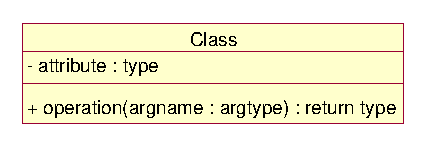
\includegraphics{umlClassIcon.eps}
        \caption{The class icon in UML.}
        \label{fig:umlClassIcon}
    \end{center}
\end{figure}
This icon is shown in Fig.~\ref{fig:umlClassIcon}.  A class icon is
simply a rectangle divided into three compartments. The topmost
show every attribute and operation of a class on any diagram.
\begin{figure}[htb]
    \begin{center}
        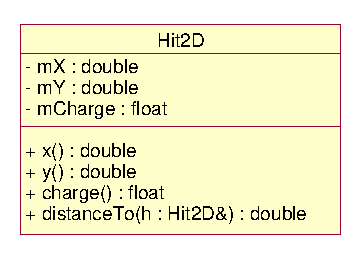
\includegraphics{umlClass.eps}
        \caption{Hit2D class. Attributes and operations are shown.}
    \end{center}
\end{figure}
Fig.~\ref{fig:umlClass} shows a typical UML description of a class
that represents a Hit (here fictitious Hit2D).  Notice that each
operations shown in italics indicate that they are pure virtual.
The corresponding C++ code for the Hit3D class from
be omitted. Notice also that the return values follow the member
functions in a similar fashion. Again, these can be omitted. Finally,
notice that the member function arguments also have a name and type.
Again one can omit the name or the arguments altogether.

At the beginning of each attribute and operations the visibility of
the class is indicated through a simple tag. UML provides three tags:
\begin{description}
\item[+] public
\item[\#] protected
\item[--] private
\end{description}
These abbreviations match exactly the three levels of visibility
provided in C++. The class shown in Fig.~\ref{fig:umlClass} is then
translated into C++ code as follows:

{\footnotesize
\begin{verbatim}
class Hit2D {
public:
Fig.~\ref{fig:umlAggregation} shows an \emph{aggregation} relationship.
    double distanceTo(Hit2D& h);
private:
    double mX, mY;
    float  mCharge;
};
\end{verbatim}
}%\footnotesize

\subsection{Composition Relationships}

Each instance of type Hit usually contains an instance of type
Position. One also says the Hit \emph{has} a Position. This is a
relationship known as composition. It can be depicted in UML using a
class relationship.  Fig.~\ref{fig:umlComposition} shows the
\emph{composition} relationship.
\begin{figure}[htb]
    \begin{center}
        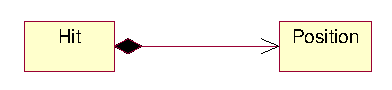
\includegraphics{umlComposition.eps}
        \caption{Class Hit has a Position.}
        \label{fig:umlComposition}
    \end{center}
\end{figure}
The black diamond represents composition. It is placed on the Hit
class because it is the Hit that is composed of (or has) a Position.
The arrowhead on the other end of the relationship denotes that the
relationship is navigable in only one direction. That is, Position
does not know about Hit. In UML relationships are presumed to be
bidirectional unless the arrowhead is present to restrict them.
Composition relationships are a strong form of containment or
aggregation. Aggregation is a whole/part relationship. In this case,
Hit is the whole, and Position is part of Hit. However, composition is
more than just aggregation. Composition also indicates that the
lifetime of Position is dependent upon Hit. This means that if Hit is
destroyed, Position will be destroyed with it.  In C++ we would
represent this as:

{\footnotesize
\begin{verbatim}
class Hit {
     Position mPos;
};
\end{verbatim}
}%\footnotesize

In this case we have represented the composition relationship as a
member variable. We could also have used a pointer so long as the
destructor of Hit deleted the pointer.  A more realistic example can
be found in \StEvent. There the \name{StHit} class has a member of
type \name{StThreeVector} which represents a position.

\subsection{Inheritance}

The inheritance relationship in UML is depicted by a triangular
arrowhead which points to the base class. One or more lines proceed
from the base of the arrowhead connecting it to the derived classes.
\begin{figure}[htb]
    \begin{center}
        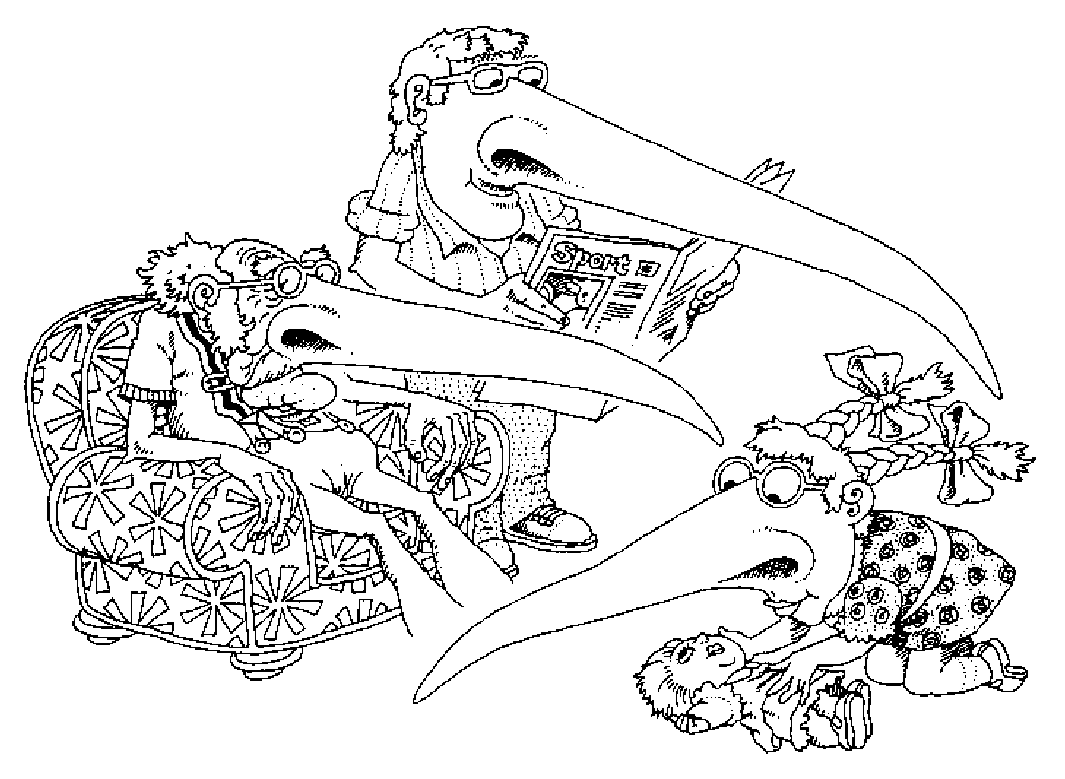
\includegraphics[width=0.7\textwidth]{cartoon6.eps}
        \caption{A subclass may inherit the structure and behaviour
            of its superclass.}
    \end{center}
\end{figure}
\begin{figure}[htb]
    \begin{center}
        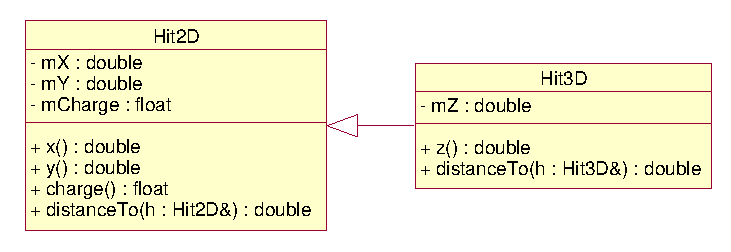
\includegraphics{umlInheritance.eps}
        \caption{Inheritance.}
        \label{fig:umlInheritance}
    \end{center}
\end{figure}

Fig.~\ref{fig:umlInheritance} shows the form of the \emph{inheritance}
relationship.  In this diagram we see that Hit3D is derived from
Hit2D.  If the name of a class would be shown in italics, it would
TrackFitter class and the CalibrartionDB class. This is the \emph{dependency}
relationship. This is often called a \emph{using} relationship.  This
relationship simply means that TrackFitter somehow depends upon
CalibrartionDB. In C++ this almost always results in a \#include:
{\footnotesize
\begin{verbatim}
class Hit3D : public Hit2D {
public:
    double z();
    double distanceTo(Hit3D& h);
private:
    double mZ;
};
\end{verbatim}
}%\footnotesize

\subsection{Aggregation and Association}

The weak form of aggregation is denoted with an open diamond. This
relationship denotes that the aggregate class (the class with the
white diamond touching it) is in some way the "whole", and the other
class in the relationship is somehow "part" of that whole.
Fig.~\ref{fig:umlAggregation} shows an \emph{aggregation}
relationship.
\begin{figure}[htb]
    \begin{center}
        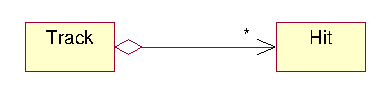
\includegraphics{umlAggregation.eps}
        \caption{Aggregation.}
        \label{fig:umlAggregation}
    \end{center}
\end{figure}
In this case, the Track class contains many Hit instances. In UML the
ends of a relationship are referred to as its "roles''. Notice that
the role at the Hit end of the aggregation is marked with a "$*$".
This indicates that the Track contains many Hit instances.  The
following Listing shows how Fig.~\ref{fig:umlAggregation} might be
implemented in C++ as:

{\footnotesize
\begin{verbatim}
class Track {
public:
    // ...
private:
    vector<Hit*> mHits;
};
\end{verbatim}
}%\footnotesize

There are other forms of containment that do not have whole/part
implications. For example, each \name{Vertex} refers back to its
parent Track. This is not aggregation since it is not reasonable to
consider a parent Track to be part of a child Vertex. We use the
\emph{association} relationship to depict this.

\begin{figure}[htb]
    \begin{center}
        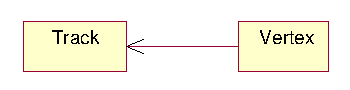
\includegraphics{umlAssociation.eps}
        \caption{Association.}
        \label{fig:umlAssociation}
    \end{center}
\end{figure}

Fig.~\ref{fig:umlAssociation} shows how we draw an association.  An
association is nothing but a line drawn between the participating
classes. In Fig.~\ref{fig:umlAssociation} the association has an
arrowhead to denote that Track does not necessarily know anything
about Vertex. This relationship will almost certainly be implemented
with a pointer of some kind.

What is the difference between an aggregation and an association?
Aggregation denotes whole/part relationships whereas associations do
not. However, there is not likely to be much difference in the way
that the two relationships are implemented.  That is, it would be very
difficult to look at the code and determine whether a particular
relationship ought to be aggregation or association.  Aggregation and
Association both correspond to the \emph{has-by-reference}
relationship.

\subsection{Dependency}

Sometimes the relationship between a two classes is very weak. They
are not implemented with member variables at all. Rather they might be
implemented as member function arguments.

Consider, for example, the fit function of a TrackFitter class.
Suppose that this function takes an argument of type CalibrartionDB
since it requires information from it (e.g. if the magnetic field was
on or off) in order to perform the fit.
\begin{figure}[htb]
    \begin{center}
        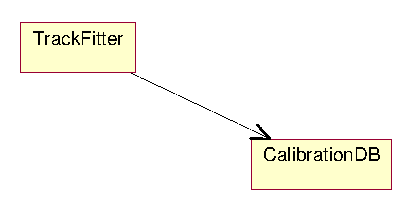
\includegraphics{umlDependency.eps}
        \caption{Dependency.}
        \label{fig:umlDependency}
    \end{center}
\end{figure}
Fig.~\ref{fig:umlDependency} shows a dashed arrow between the
TrackFitter class and the CalibrartionDB class. This is the
\emph{dependency} relationship. This is often called a \emph{using}
relationship.  This relationship simply means that TrackFitter somehow
depends upon CalibrartionDB. In C++ this almost always results in a
\#include:

{\footnotesize
\begin{verbatim}
#include "CalibrartionDB.hh"
class TrackFitter {
public:
    // ...
    void fit(CalibrartionDB &db);
private:
    // ...
};
\end{verbatim}
}%\footnotesize

%%%%%%%%%%%%%%%%%%%%%%%%%%%%%%%%%%%%%%%%%%%%%%%%%%%%%%%%%%%%%%%%%%%%
%
% The End
%
%%%%%%%%%%%%%%%%%%%%%%%%%%%%%%%%%%%%%%%%%%%%%%%%%%%%%%%%%%%%%%%%%%%%

\printindex

\end{document}
\bye
% The text following after this line is not included into the text

%
%  Template for reference section
%

%%%%%%%%%%%%%%%%%%%%%%%%%%%%%%%%%%%%%%%%%%%%%%%%%%%%%%%%%%%%%%%%%%%%
%
%    Reference: className
%
%%%%%%%%%%%%%%%%%%%%%%%%%%%%%%%%%%%%%%%%%%%%%%%%%%%%%%%%%%%%%%%%%%%%
\subsection{className}
\index{className|textbf}
\label{sec:className}
\begin{Entry}
\item[Summary]

\item[Synopsis]
    \verb+#include "className.hh"+\\
    \verb+class className;+\\

\item[Description]

\item[Persistence]
    None

\item[Related Classes]

\item[Public\\ Constructors]

\item[Public Member\\ Functions]

\item[Public Member\\ Operators]

\item[Public Functions]

\item[Public Operators]

\item[Examples]
{\footnotesize
\begin{verbatim}
//
//  What the example does
//

\end{verbatim}
}%footnotesize

\end{Entry}
